% 第 3 章：抛物不动点：Fatou 坐标与 horn 映射
% 本章新增宏（\providecommand，见汇报）
\providecommand{\Patt}{P_{\mathrm{att}}}
\providecommand{\Prep}{P_{\mathrm{rep}}}
\providecommand{\Oatt}{\Omega_{\mathrm{att}}}
\providecommand{\Orep}{\Omega_{\mathrm{rep}}}
\providecommand{\lrep}{\ell_{\mathrm{rep}}}
\providecommand{\Arg}{\operatorname{Arg}}

\chapter{抛物不动点：Fatou 坐标与 horn 映射}\label{ch:fatou}

第~\ref{ch:koenigs}~章处理了双曲不动点：在乘子满足 $0<|\lambda|\ne1$ 的不动点附近，Koenigs 坐标把映射线性化，
取对数后得到 Abel 方程 $\Phi\circ f=\Phi+1$ 的解。当两个实不动点在鞍结中合并时，
乘子趋于 $1$，Koenigs 坐标退化。本章研究极限情形本身：一个乘子为 $1$ 的不动点，
即\textbf{抛物不动点}（parabolic fixed point）。

在抛物点附近，Abel 方程仍然有解，但解不再在整个邻域上存在，而是分别存在于两片
\textbf{花瓣}（petal）上：吸引花瓣上的 $\Phiatt$ 和排斥花瓣上的 $\Phirep$。两片花瓣
在不动点的上方和下方各有一个公共区域。在公共区域里比较两个坐标，得到一个与平移
$z\mapsto z+1$ 交换的映射，即 \textbf{horn 映射}（horn map）。它的 Fourier 系数 $B_n$
是芽在解析共轭下的不变量，也是本书后半部分的核心数据：第 7 章将证明，鞍结开折
在双曲一侧的转移映射不变量 $\tau_n$ 收敛到 $B_n\ee^{2\pi\ii na}$。

本章对一般的二重抛物芽 $g(u)=u+a_2u^2+a_3u^3+\cdots$（$a_2>0$）展开全部论证，
不使用指数函数的任何特殊性质。

\begin{goals}
\item 在坐标 $\zeta=-1/(a_2u)$ 中，$g$ 近似于平移 $\zeta\mapsto\zeta+1$；由此证明二重情形的 Leau--Fatou 花瓣定理，以及轨道渐近 $g^n(u)\approx-1/(a_2n)$。
\item 形式 Abel 函数 $\alpha(u)=-1/(a_2u)+\rho\log(-u)+\sum d_ku^k$ 存在且在相差常数的意义下唯一；迭代留数 $\rho=1-a_3/a_2^2$ 是形式共轭不变量。
\item Fatou 坐标 $\Phiatt$、$\Phirep$ 存在、单叶，并且用 $\alpha$ 归一化之后唯一。
\item 逆 horn 映射 $\horn^{-1}=\Phiatt\circ\Phirep^{-1}=z+\sum_{n\ge1}B_n\ee^{2\pi\ii nz}$ 没有常数项；逆下 horn 映射的常数项是 $2\pi\ii\rho$；乘积 $B_n\ee^{2\pi\ii na}$ 不依赖坐标的选取。
\item 当直接吸引域只含一个奇异值时 $B_1\ne0$；两个算例 $\ee^u-1$ 与 $u+u^2$ 的数值。
\end{goals}

%======================================================================
\section{二重抛物芽与坐标 \texorpdfstring{$\zeta$}{zeta}}\label{ch3:sec:germ}

\begin{definition}[二重抛物芽]\label{ch3:def:germ}
设 $g$ 在圆盘 $D_r=\{|u|<r\}$ 上全纯且单叶，
\[
 g(u)=u+a_2u^2+a_3u^3+O(u^4),\qquad a_2>0 .
\]
称 $g$ 是一个\textbf{二重抛物芽}（parabolic germ of multiplicity two），称
\[
 \rho:=1-\frac{a_3}{a_2^2}
\]
为它的\textbf{迭代留数}（iterative residue，法文 résidu itératif）。若 $g$ 的 Taylor
系数都是实数，称 $g$ 为\textbf{实芽}。
\end{definition}

条件 $a_2\ne0$ 说明 $0$ 是 $g(u)-u$ 的二重零点，即 $0$ 作为不动点的重数为 $2$。
若 $a_2\ne0$ 是任意复数，用 $u\mapsto cu$ 把它变成正数即可；本书的芽来自实鞍结开折
（第~\ref{ch:unfolding}~章），其中 $a_2>0$ 是自然的正规化。我们保留 $a_2$ 而不把它缩放为
$1$，因为第 4--9 章的公式要用到它。

逆映射 $g^{-1}$ 在 $0$ 的某个邻域上有定义，并且
\begin{equation}\label{ch3:eq:ginv}
 g^{-1}(u)=u-a_2u^2+(2a_2^2-a_3)u^3+O(u^4).
\end{equation}
（把 $u=v-a_2v^2+bv^3$ 代入 $g$ 并比较 $v^3$ 的系数，得 $b=2a_2^2-a_3$。）

\begin{lemma}[坐标 $\zeta$]\label{ch3:lem:zeta}
令 $\zeta=-1/(a_2u)$，并记
\[
 G(\zeta):=-\frac{1}{a_2\,g\bigl(-1/(a_2\zeta)\bigr)} .
\]
存在 $R_1>0$ 与 $C_1>0$，使得 $G$ 和 $G^{-1}$ 在 $\{|\zeta|>R_1\}$ 上全纯、单叶，并且
\begin{equation}\label{ch3:eq:G}
 \Bigl|G(\zeta)-\zeta-1-\frac{\rho}{\zeta}\Bigr|\le\frac{C_1}{|\zeta|^2},\qquad
 \Bigl|G^{-1}(\zeta)-\zeta+1+\frac{\rho}{\zeta}\Bigr|\le\frac{C_1}{|\zeta|^2}
 \qquad(|\zeta|>R_1).
\end{equation}
\end{lemma}

\begin{proof}
缩小 $r$，可设 $g(u)=u\bigl(1+x(u)\bigr)$，$x(u)=a_2u+a_3u^2+u^3k(u)$，其中 $k$ 在
$D_r$ 上有界，且 $|x(u)|\le1/2$。于是
$G(\zeta)=\zeta/(1+x)$，而
$\frac{1}{1+x}=1-x+x^2-\frac{x^3}{1+x}$。由 $a_2u=-1/\zeta$，
\[
 x=-\frac1\zeta+\frac{a_3}{a_2^2\zeta^2}+O(|\zeta|^{-3}),\qquad
 \frac1{1+x}=1+\frac1\zeta+\frac{1}{\zeta^2}-\frac{a_3}{a_2^2\zeta^2}+O(|\zeta|^{-3}).
\]
乘以 $\zeta$ 得 $G(\zeta)=\zeta+1+\rho/\zeta+O(|\zeta|^{-2})$，其中 $O$ 的常数只依赖于
$a_2$、$a_3$ 和 $\sup|k|$。对 $g^{-1}$ 用 \eqref{ch3:eq:ginv} 作同样的计算：此时
$x=1/\zeta+(2a_2^2-a_3)/(a_2^2\zeta^2)+O(|\zeta|^{-3})$，
$\zeta/(1+x)=\zeta-1+(1-2+a_3/a_2^2)/\zeta+O(|\zeta|^{-2})=\zeta-1-\rho/\zeta+O(|\zeta|^{-2})$。
单叶性来自 $g$、$g^{-1}$ 的单叶性和 $u\mapsto\zeta$ 是 Möbius 变换。
\end{proof}

由 \eqref{ch3:eq:G}，存在 $C_2$ 使 $|G(\zeta)-\zeta-1|\le C_2/|\zeta|$，
$|G^{-1}(\zeta)-\zeta+1|\le C_2/|\zeta|$。固定 $R_*\ge\sqrt2\max(R_1,\,4C_2,\,10)$。
于是当 $|\zeta|\ge R_*/\sqrt2$ 时
\begin{equation}\label{ch3:eq:quarter}
 |G(\zeta)-\zeta-1|\le\tfrac14,\qquad |G^{-1}(\zeta)-\zeta+1|\le\tfrac14,\qquad
 \Bigl|\frac{G(\zeta)}{\zeta}-1\Bigr|\le\frac{5}{4|\zeta|}\le\frac{1}{5}.
\end{equation}

\begin{example}\label{ch3:ex:zeta}
(1) $g(u)=u+u^2$：$a_2=1$，$a_3=0$，$\rho=1$。此时 $G$ 可以精确算出：
$G(\zeta)=-1/(u(1+u))=\zeta^2/(\zeta-1)=\zeta+1+\frac{1}{\zeta-1}$。

(2) $g(u)=\ee^u-1=u+\tfrac12u^2+\tfrac16u^3+\cdots$：$a_2=\tfrac12$，$a_3=\tfrac16$，
$\rho=1-\tfrac{1/6}{1/4}=\tfrac13$，$\zeta=-2/u$，
$G(\zeta)=-2/(\ee^{-2/\zeta}-1)=\zeta+1+\frac{1}{3\zeta}+O(\zeta^{-3})$
（展开 $x/(\ee^x-1)$ 的 Bernoulli 级数可知 $\zeta^{-2}$ 项为零）。这是 tetration 在
$b=\eta=\ee^{1/\ee}$ 处的芽：在 $w=\ee(1+u)$ 中，$w\mapsto\eta^w$ 变成 $u\mapsto\ee^u-1$
（\cite[\S2.1]{KneserPaper}）。

(3) $g(u)=u/(1-u)=u+u^2+u^3+\cdots$：$\rho=0$，且 $G(\zeta)=\zeta+1$ 恰为平移。
\end{example}

%======================================================================
\section{Leau--Fatou 花瓣}\label{ch3:sec:petals}

记
\[
 s(\zeta):=\Rea\zeta+|\Ima\zeta|,\qquad t(\zeta):=-\Rea\zeta+|\Ima\zeta| .
\]

\begin{definition}[花瓣]\label{ch3:def:petals}
对 $R\ge R_*$，令
\[
 \Oatt(R)=\{\zeta:\ s(\zeta)>R\},\qquad \Orep(R)=\{\zeta:\ t(\zeta)>R\},
\]
并称它们在 $u$ 平面中的原像
$\Patt(R)=\{u\ne0:\ -1/(a_2u)\in\Oatt(R)\}$、
$\Prep(R)=\{u\ne0:\ -1/(a_2u)\in\Orep(R)\}$
为\textbf{吸引花瓣}与\textbf{排斥花瓣}（attracting / repelling petal）。
\end{definition}

$\Oatt(R)$ 是平面去掉一个顶点在 $R$、开口向左、张角 $\pi/2$ 的闭角形区域；
$\Orep(R)=-\Oatt(R)$。$\Oatt(R)$ 是两个半平面 $\{\Rea\zeta\pm\Ima\zeta>R\}$ 之并，所以在 $u$ 平面中，
$\Patt(R)$ 是两个边界过原点的开圆盘之并，含有负实轴的一段，见\cref{ch3:fig:petals}(a)。下面几条初等事实反复使用：
\begin{enumerate}[label=(\alph*)]
\item $s(\zeta)\le|\Rea\zeta|+|\Ima\zeta|\le\sqrt2|\zeta|$，同样 $t(\zeta)\le\sqrt2|\zeta|$；
\item $\Oatt(R)\subset\{|\Arg\zeta|<3\pi/4\}$，$\Orep(R)\subset\{|\Arg(-\zeta)|<3\pi/4\}$，其中 $\Arg$ 是主值辐角；
\item $\Oatt(R)\cup\Orep(R)=\{|\Rea\zeta|+|\Ima\zeta|>R\}\supset\{|\zeta|>R\}$；
\item $\Oatt(R)\cap\Orep(R)=\{|\Ima\zeta|>R+|\Rea\zeta|\}$，它有两个连通分支 $W_+(R)\subset\{\Ima\zeta>0\}$、$W_-(R)\subset\{\Ima\zeta<0\}$。
\end{enumerate}
(b) 的理由：若 $\zeta\in\Oatt(R)$ 且 $\Rea\zeta<0$，则 $|\Ima\zeta|>R+|\Rea\zeta|>|\Rea\zeta|$。
(c) 的理由：$\max(s,t)=|\Rea\zeta|+|\Ima\zeta|$。注意 $\zeta$ 与 $u$ 的上下半平面一致：
$-1/u$ 把上半平面映为上半平面，所以 $\Ima\zeta>0\iff\Ima u>0$。

\begin{theorem}[Leau--Fatou 花瓣定理，二重情形]\label{ch3:thm:flower}
设 $g$ 是二重抛物芽，$R\ge R_*$。
\begin{enumerate}
\item $G(\Oatt(R))\subset\Oatt(R)$，且 $s(G(\zeta))\ge s(\zeta)+\tfrac12$；
 $G^{-1}(\Orep(R))\subset\Orep(R)$，且 $t(G^{-1}(\zeta))\ge t(\zeta)+\tfrac12$。
\item 对 $u\in\Patt(R)$ 和 $n\ge0$，$|g^n(u)|\le\sqrt2/\bigl(a_2(R+n/2)\bigr)$；特别地 $g^n\to0$ 在 $\Patt(R)$ 上一致成立。对 $\Prep(R)$ 与 $g^{-n}$ 有同样的结论。
\item $\Patt(R)\cup\Prep(R)\cup\{0\}\supset D_{1/(a_2R)}$。
\item 若 $u\ne0$，$g^n(u)\to0$ 且对所有 $n$ 有 $g^n(u)\ne0$，则 $n$ 充分大时 $g^n(u)\in\Patt(R)$。对后向轨道与 $\Prep(R)$ 有同样的结论。
\item 对 $u\in\Patt(R)$，$n\,g^n(u)\to-1/a_2$，且 $\Arg(-g^n(u))\to0$；收敛关于 $u$ 在 $\Patt(R)$ 的紧子集上一致。即轨道沿负实轴方向切向地趋于 $0$，并且 $g^n(u)\approx-1/(a_2n)$。
\end{enumerate}
\end{theorem}

\begin{proof}
(1) 若 $\zeta\in\Oatt(R)$，由 (a) 有 $|\zeta|\ge s(\zeta)/\sqrt2>R_*/\sqrt2$，于是
\eqref{ch3:eq:quarter} 给出 $\Rea G(\zeta)\ge\Rea\zeta+\tfrac34$，
$|\Ima G(\zeta)|\ge|\Ima\zeta|-\tfrac14$，相加得 $s(G(\zeta))\ge s(\zeta)+\tfrac12$。
排斥一侧同理。

(2) 由 (1)，$s(G^n\zeta)\ge R+n/2$，再由 (a)，$|G^n\zeta|\ge(R+n/2)/\sqrt2$，而
$|g^n(u)|=1/(a_2|G^n\zeta|)$。

(3) 由 (c)：$|u|<1/(a_2R)$ 等价于 $|\zeta|>R$。

(4) 记 $\zeta_n=-1/(a_2g^n(u))$，则 $\zeta_n\to\infty$，故对 $n\ge n_0$ 有 $|\zeta_n|>R$，从而
$\zeta_n\in\Oatt(R)\cup\Orep(R)$。若某个 $\zeta_n\in\Oatt(R)$，由 (1) 以后都在其中。
否则对所有 $n\ge n_0$，$\zeta_n\in\Orep(R)$，且 $\zeta_n=G^{-1}(\zeta_{n+1})$，由 (1)
$t(\zeta_n)\ge t(\zeta_{n+1})+\tfrac12$。于是 $t(\zeta_n)\le t(\zeta_{n_0})-(n-n_0)/2\to-\infty$，
与 $t(\zeta_n)>R$ 矛盾。后向轨道的论证对称。

(5) 记 $\zeta_k=G^k\zeta$。由 $|G(\zeta)-\zeta-1|\le C_2/|\zeta|$ 和 (2)，
\[
 |\zeta_n-\zeta-n|\le\sum_{k<n}\frac{C_2}{|\zeta_k|}
 \le\sqrt2C_2\sum_{k<n}\frac{1}{R+k/2}
 \le\sqrt2C_2\Bigl(\frac1R+2\log\Bigl(1+\frac{n}{2R}\Bigr)\Bigr).
\]
所以 $\zeta_n=n+O(\log n)$，$O$ 在 $\zeta$ 的有界集上一致。于是
$n\,g^n(u)=-n/(a_2\zeta_n)\to-1/a_2$；又 $\Rea\zeta_n\ge n/2$、$\Ima\zeta_n=O(\log n)$，故
$\Arg\zeta_n\to0$，而 $\Arg(-g^n(u))=-\Arg\zeta_n$。
\end{proof}

更精确的渐近式（含 $\log n/n^2$ 项）要用到 Fatou 坐标，见\cref{ch3:cor:orbit}。

\begin{definition}[抛物吸引域]\label{ch3:def:basin}
设 $g$ 是整函数 $f$ 在 $0$ 处的芽。称
$\mathfrak B=\{u\in\C:\ \text{存在 }n\ge0\text{ 使 }f^n(u)\in\Patt(R)\}$
为 $0$ 的\textbf{抛物吸引域}（parabolic basin），称 $\mathfrak B$ 中含 $\Patt(R)$ 的连通分支
$\mathcal A$ 为\textbf{直接吸引域}（immediate basin）。
\end{definition}

由\cref{ch3:thm:flower}(4)，$\mathfrak B$ 恰为满足 $f^n(u)\to0$ 且 $f^n(u)\ne0$ 的点集，
因此与 $R$ 无关；$\Patt(R)$ 连通，所以 $\mathcal A$ 也与 $R$ 无关。显然
$f^{-1}(\mathfrak B)=\mathfrak B$。

\begin{remark}[实芽的实吸引区间]\label{ch3:rem:real-basin}
设 $f$ 是实整函数，$\ustar<0$，且在 $[\ustar,0)$ 上 $f$ 递增并满足 $f(u)>u$。
则对 $u\in[\ustar,0)$，$u<f(u)<f(0)=0$，所以轨道严格递增且有上界 $0$，其极限是
$[\ustar,0]$ 中的不动点；$[\ustar,0)$ 中没有不动点，故极限为 $0$。因此
$[\ustar,0)\subset\mathcal A$。这正是第 4 章假设 (H4) 中基点所处的位置
（\cref{def:unfolding}）。对 $\ee^u-1$，整条负实轴都在 $\mathcal A$ 中。对 $u+u^2$，上述条件在 $[-\tfrac12,0)$ 上成立；
$f$ 把 $(-1,0)$ 映入 $[-\tfrac14,0)$，所以整个区间 $(-1,0)$ 在 $\mathcal A$ 中。
\end{remark}

%======================================================================
\section{形式 Abel 函数与迭代留数}\label{ch3:sec:formal}

我们要找 Abel 方程 $\alpha\circ g=\alpha+1$ 的形式解。由\cref{ch3:lem:zeta}，在 $\zeta$
坐标中 $G(\zeta)=\zeta+1+\rho/\zeta+O(\zeta^{-2})$。令 $\chi(\zeta)=\zeta-\rho\log\zeta$，则
$\chi(G(\zeta))=\zeta+1+\frac\rho\zeta-\rho\log\zeta-\rho\log\bigl(1+\frac1\zeta+O(\zeta^{-2})\bigr)=\chi(\zeta)+1+O(\zeta^{-2})$。这提示首项应为
$\zeta-\rho\log\zeta=-1/(a_2u)+\rho\log(-u)+\text{常数}$。

\textbf{形式框架。} 考虑形如
\begin{equation}\label{ch3:eq:class}
 \beta(u)=\frac{A}{u}+c\log(-u)+\varphi(u),\qquad A,c\in\C,\ \varphi\in\C[[u]]
\end{equation}
的形式表达式。对二重抛物芽 $g$（这里只用它的 Taylor 级数），定义
\[
 \beta\circ g-\beta:=A\Bigl(\frac1{g(u)}-\frac1u\Bigr)+c\,L_g(u)+\bigl(\varphi\circ g-\varphi\bigr),
 \qquad L_g(u):=\log\frac{g(u)}{u}\in u\C[[u]] ,
\]
其中 $L_g$ 是 $\log(1+a_2u+a_3u^2+\cdots)$ 的形式展开。因为
\begin{equation}\label{ch3:eq:inv-diff}
 \frac1{g}-\frac1u=\frac{u-g}{ug}=-\frac{a_2+a_3u+\cdots}{1+a_2u+\cdots}
 =-a_2+(a_2^2-a_3)u+O(u^2),
\end{equation}
$\beta\circ g-\beta$ 是 $\C[[u]]$ 中的元素。这一定义与收敛情形一致：若 $\log(-u)$
沿着从 $u$ 到 $g(u)$ 的短线段连续延拓，则 $\log(-g(u))-\log(-u)=\log(g(u)/u)$
（见\cref{ch3:lem:defect}）。

\begin{lemma}[差分算子]\label{ch3:lem:Delta}
记 $\Delta\varphi=\varphi\circ g-\varphi$。则对 $k\ge1$，
$\Delta(u^k)=ka_2u^{k+1}+O(u^{k+2})$，并且 $\Delta$ 是从 $u\C[[u]]$ 到 $u^2\C[[u]]$ 的线性
双射。$\Delta$ 在 $\C[[u]]$ 上的核是常数。
\end{lemma}

\begin{proof}
$g^k-u^k=u^k\bigl((1+a_2u+\cdots)^k-1\bigr)=ka_2u^{k+1}+O(u^{k+2})$。对
$\varphi=\sum_{k\ge1}\varphi_ku^k$，$\Delta\varphi$ 的 $u^{m+1}$ 项系数等于
$ma_2\varphi_m$ 加上只含 $\varphi_1,\dots,\varphi_{m-1}$ 的线性组合。这是对角元
$ma_2\ne0$ 的下三角无穷线性方程组，所以对任意右端 $\sum_{m\ge1}r_{m+1}u^{m+1}$ 可逐阶
唯一解出 $\varphi_1,\varphi_2,\dots$。常数显然在核中，而 $u\C[[u]]$ 中的核为零。
\end{proof}

\begin{theorem}[形式 Abel 函数]\label{ch3:thm:formal}
设 $g$ 是二重抛物芽。
\begin{enumerate}
\item 在形如 \eqref{ch3:eq:class} 的表达式中，满足 $\beta\circ g-\beta=1$ 的解必有
 $A=-1/a_2$、$c=\rho$。
\item 存在唯一的 $\varphi\in u\C[[u]]$（即无常数项），使
 $\alpha(u)=-\frac1{a_2u}+\rho\log(-u)+\varphi(u)$ 满足 $\alpha\circ g=\alpha+1$；
 \eqref{ch3:eq:class} 中的全部解是 $\alpha+\text{常数}$。
\item 若 $g$ 是实芽，则 $\varphi$ 的系数都是实数。
\end{enumerate}
\end{theorem}

\begin{definition}[形式 Abel 函数]\label{def:formal-abel}
\Cref{ch3:thm:formal}(2) 中的
\[
 \alpha(u)=-\frac{1}{a_2u}+\rho\log(-u)+\sum_{k\ge1}d_ku^k,\qquad \alpha\circ g=\alpha+1,
\]
称为 $g$ 的\textbf{形式 Abel 函数}（formal Abel function）；它的归一化是幂级数部分没有常数项。
记它的截断为
\[
 \alpha_N(u)=-\frac{1}{a_2u}+\rho\log(-u)+\sum_{k=1}^Nd_ku^k\qquad(N\ge0),
\]
特别地 $\alpha_0(u)=-1/(a_2u)+\rho\log(-u)$。$\log(-u)$ 取哪个分支，要等到它作为函数
使用时（\cref{ch3:sec:fatou}）才规定。
\end{definition}

\begin{proof}[\cref{ch3:thm:formal} 的证明]
(1) 由 \eqref{ch3:eq:inv-diff} 和 $L_g=a_2u+O(u^2)$，并由\cref{ch3:lem:Delta}
（$\Delta\varphi\in u^2\C[[u]]$），
\[
 \beta\circ g-\beta=-Aa_2+\bigl(A(a_2^2-a_3)+ca_2\bigr)u+O(u^2).
\]
令它等于 $1$：常数项给出 $A=-1/a_2$；$u$ 项给出
$c=-A(a_2^2-a_3)/a_2=1-a_3/a_2^2=\rho$。

(2) 取 $A=-1/a_2$、$c=\rho$，方程化为
$\Delta\varphi=r$，$r:=1+\frac{1}{a_2}\bigl(\frac1g-\frac1u\bigr)-\rho L_g$。由 (1) 的计算，
$r$ 的常数项和 $u$ 项都是零，即 $r\in u^2\C[[u]]$。由\cref{ch3:lem:Delta}，在 $u\C[[u]]$
中有唯一解；全部解相差 $\Delta$ 的核，即常数。

(3) 实芽时 $r$ 的系数是实数，三角方程组的解也是实数。
\end{proof}

逐阶求解给出系数的显式公式。例如（习题~\ref{ch3:exe:d1}）
\begin{equation}\label{ch3:eq:d1}
 d_1=\frac{2a_3^2+a_2^2a_3-2a_2a_4-a_2^4}{2a_2^3}.
\end{equation}

\begin{example}[两个形式 Abel 函数]\label{ch3:ex:formal}
用 \texttt{sympy} 逐阶求解（与 \texttt{docs/generality\_check.py} 中 \texttt{Alpha} 类的
浮点输出一致）：
\begin{align*}
 \ee^u-1:&\quad \alpha(u)=-\frac2u+\frac13\log(-u)-\frac{u}{36}+\frac{u^2}{540}+\frac{u^3}{7776}-\frac{71\,u^4}{435456}+\cdots,\\
 u+u^2:&\quad \alpha(u)=-\frac1u+\log(-u)-\frac{u}{2}+\frac{u^2}{3}-\frac{13\,u^3}{36}+\frac{113\,u^4}{240}+\cdots.
\end{align*}
第一行即论文的 \cite[\S2.1]{KneserPaper} 中的展开（论文记系数为 $c^\alpha_k$）。对
$g(u)=u/(1-u)$，$\alpha(u)=-1/u$ 精确成立。
\end{example}

\begin{proposition}[迭代留数是形式不变量]\label{ch3:prop:rho-invariant}
设 $h(v)=cv+O(v^2)\in\C[[v]]$，$c\ne0$，$\tilde g:=h^{-1}\circ g\circ h$（形式复合）。则
$\tilde g(v)=v+\tilde a_2v^2+\tilde a_3v^3+\cdots$，$\tilde a_2=ca_2$，并且
$\tilde\rho:=1-\tilde a_3/\tilde a_2^2=\rho$。
\end{proposition}

\begin{proof}
$\tilde a_2=ca_2$ 由比较 $v^2$ 系数得到。考虑 $\alpha\circ h$，其中
$\log(-h(v))$ 按 $\log(-v)+\log c+\log\bigl(h(v)/(cv)\bigr)$ 理解（$\log c$ 取定任一值）。
写 $h(v)=cv(1+e_1v+\cdots)$，则
\[
 \alpha(h(v))=-\frac{1}{a_2cv}(1-e_1v+\cdots)+\rho\log(-v)+\rho\log c+O(v)
 =-\frac{1}{\tilde a_2v}+\rho\log(-v)+\tilde\varphi(v),
\]
$\tilde\varphi\in\C[[v]]$。另一方面
$(\alpha\circ h)\circ\tilde g=\alpha\circ g\circ h=\alpha\circ h+1$，所以 $\alpha\circ h$ 是
$\tilde g$ 的、形如 \eqref{ch3:eq:class} 的 Abel 方程的解。由\cref{ch3:thm:formal}(1)，
其对数项系数等于 $\tilde\rho$。故 $\tilde\rho=\rho$。
\end{proof}

\begin{remark}[形式分类]\label{ch3:rem:formal-class}
\Cref{ch3:prop:rho-invariant} 的逆命题也成立：两个 $a_2$ 相同的二重抛物芽在形式上
通过切于恒等的变换共轭，当且仅当它们的迭代留数相同。一个标准代表是向量场
$X_{a_2,\rho}=\frac{a_2u^2}{1+\rho a_2u}\,\partial_u$ 的时间一映射；它的时间函数恰好是
$-1/(a_2u)+\rho\log(-u)$（习题~\ref{ch3:exe:normal-form}）。因此形式理论里只有
$(a_2,\rho)$ 两个不变量，而 $a_2$ 可以用缩放消去。下面将看到，解析分类需要无穷多个
额外的不变量，即 horn 映射。
\end{remark}

\begin{remark}[发散性]\label{ch3:rem:divergence}
级数 $\sum d_ku^k$ 一般是发散的。对 $\ee^u-1$ 和 $u+u^2$，这将由 $B_1\ne0$ 推出
（\cref{ch3:cor:divergence}）。Écalle 证明了它是 Borel 可和的，其 Stokes 现象恰好由
horn 映射描述 \cite{Ecalle1981,DudkoSauzin2014}；本书不用这一事实。
\end{remark}

%======================================================================
\section{Fatou 坐标}\label{ch3:sec:fatou}

\subsection{对数的分支与单步误差}
在吸引花瓣上，$\zeta\in\Oatt(R)\subset\{|\Arg\zeta|<3\pi/4\}$，而 $-u=1/(a_2\zeta)$，
所以 $|\Arg(-u)|<3\pi/4$。我们在 $\Patt(R)$ 上用主值 $\Log(-u)$。在排斥花瓣上
$|\Arg u|<3\pi/4$，我们用
\begin{equation}\label{ch3:eq:lrep}
 \lrep(u):=\Log u-\ii\pi\qquad(u\in\Prep(R)).
\end{equation}
它是 $\log(-u)$ 在 $\Prep(R)$ 上的一个连续分支，并且在上半平面与主值 $\Log(-u)$ 相同，
在下半平面等于 $\Log(-u)-2\pi\ii$。相应地记
\[
 \alpha_N^{\mathrm{att}}(u)=-\frac1{a_2u}+\rho\Log(-u)+\sum_{k=1}^Nd_ku^k,\qquad
 \alpha_N^{\mathrm{rep}}(u)=-\frac1{a_2u}+\rho\,\lrep(u)+\sum_{k=1}^Nd_ku^k .
\]
在 $\zeta$ 坐标中，$\alpha_0^{\mathrm{att}}=\zeta-\rho\Log\zeta-\rho\log a_2$
（因为 $a_2>0$ 且 $\zeta\notin(-\infty,0]$）。

\begin{lemma}[单步误差]\label{ch3:lem:defect}
缩小 $r$ 使 $|g(u)/u-1|<1/5$ 在 $D_r$ 上成立。对 $N\ge0$ 令
\[
 E_N(u):=\frac{1}{a_2u}-\frac{1}{a_2g(u)}+\rho\Log\frac{g(u)}{u}
 +\sum_{k=1}^Nd_k\bigl(g(u)^k-u^k\bigr)-1 .
\]
则 $E_N$ 在 $D_r$ 上全纯（$0$ 是可去奇点），并存在 $M_N$ 使
$|E_N(u)|\le M_N|u|^{N+2}$（$|u|\le r/2$）。若 $R$ 充分大，则对 $u\in\Patt(R)$ 有
$\alpha_N^{\mathrm{att}}(g(u))-\alpha_N^{\mathrm{att}}(u)-1=E_N(u)$；对 $u,g(u)\in\Prep(R)$ 有
$\alpha_N^{\mathrm{rep}}(g(u))-\alpha_N^{\mathrm{rep}}(u)-1=E_N(u)$。
\end{lemma}

\begin{proof}
由 \eqref{ch3:eq:inv-diff}，$1/u-1/g(u)$ 在 $0$ 处可去；$g(u)/u$ 在 $D_r$ 上取值于
$\{|w-1|<1/5\}$，其主值对数全纯。所以 $E_N$ 全纯，其 Taylor 级数等于形式表达式
$\alpha_N\circ g-\alpha_N-1$。由于 $\alpha\circ g-\alpha-1=0$，
\[
 \alpha_N\circ g-\alpha_N-1=-\Delta\Bigl(\sum_{k>N}d_ku^k\Bigr)\in u^{N+2}\C[[u]]
\]
（\cref{ch3:lem:Delta}）。故 $E_N(u)/u^{N+2}$ 在 $D_r$ 上全纯，在 $\overline{D_{r/2}}$ 上有界。

对分支：若 $u\in\Patt(R)$，则 $g(u)\in\Patt(R)$（\cref{ch3:thm:flower}(1)），
$\Arg(-u)$、$\Arg(-g(u))$ 都在 $(-3\pi/4,3\pi/4)$ 中，其差在 $(-3\pi/2,3\pi/2)$ 中，
且模 $2\pi$ 同余于 $\Arg(g(u)/u)$，而 $|\Arg(g(u)/u)|<\pi/4$。若二者不相等，差至少为
$2\pi-\pi/4>3\pi/2$，不可能。所以 $\Log(-g(u))-\Log(-u)=\Log(g(u)/u)$。排斥一侧把
$\Arg(-\cdot)$ 换成 $\Arg(\cdot)$，论证相同。
\end{proof}

\begin{lemma}[轨道求和]\label{ch3:lem:sum}
设 $R\ge R_*$，$m\ge2$。对 $u\in\Patt(R)$，$\zeta=-1/(a_2u)$，
\[
 \sum_{k\ge0}|g^k(u)|^m\le3\Bigl(\frac{\sqrt2}{a_2}\Bigr)^m s(\zeta)^{1-m}.
\]
对 $u\in\Prep(R)$，把 $g^k$ 换成 $g^{-k}$、$s$ 换成 $t$，结论相同。
\end{lemma}

\begin{proof}
由\cref{ch3:thm:flower}(1) 和 (a)，$|g^k(u)|\le\sqrt2/(a_2(s+k/2))$，$s=s(\zeta)\ge R_*\ge1$。而
$\sum_{k\ge0}(s+k/2)^{-m}\le s^{-m}+\int_0^\infty(s+x/2)^{-m}\dd x=s^{-m}+\frac{2s^{1-m}}{m-1}\le3s^{1-m}$。
\end{proof}

\subsection{存在性、唯一性与单叶性}

\begin{theorem}[Fatou 坐标]\label{thm:fatou-coordinates}
设 $g$ 是二重抛物芽，$\alpha$ 是它的形式 Abel 函数。存在 $R_0\ge R_*$，使对 $R\ge R_0$：
\begin{enumerate}
\item （存在）对每个 $N\ge0$，极限
 \[
  \Phiatt(u):=\lim_{n\to\infty}\bigl[\alpha_N^{\mathrm{att}}(g^n(u))-n\bigr]
 \]
 在 $\Patt(R)$ 上一致存在且与 $N$ 无关；$\Phiatt$ 在 $\Patt(R)$ 上全纯，
 $\Phiatt\circ g=\Phiatt+1$。
\item （渐近）存在常数 $K_N$，使
 $|\Phiatt(u)-\alpha_N^{\mathrm{att}}(u)|\le K_N\,s(\zeta)^{-N-1}$，$\zeta=-1/(a_2u)$。
 特别地，对每个 $\delta>0$，当 $u\to0$ 且 $|\Arg(-u)|\le3\pi/4-\delta$ 时，
 $\Phiatt(u)=\alpha_N^{\mathrm{att}}(u)+O(|u|^{N+1})$；即 $\Phiatt$ 以 $\alpha$ 为渐近展开。
\item （单叶）$\Phiatt$ 在 $\Patt(R)$ 上单叶；对每个 $w\in\C$，当 $n$ 充分大时
 $w+n\in\Phiatt(\Patt(R))$。
\item （唯一）若 $\Phi$ 在 $\Patt(R)$ 上全纯，$\Phi\circ g=\Phi+1$，且
 $\Phi-\alpha_0^{\mathrm{att}}$ 在 $\Patt(R)$ 上有界，则 $\Phi-\Phiatt$ 是常数；若再有
 某个 $u$ 使 $\Phi(g^nu)-\alpha_0^{\mathrm{att}}(g^nu)\to0$，则 $\Phi=\Phiatt$。
\item （排斥坐标）在 $\Prep(R)$ 上，
 $\Phirep(u):=\lim_{n\to\infty}\bigl[\alpha_N^{\mathrm{rep}}(g^{-n}(u))+n\bigr]$
 存在、全纯、单叶，满足 $\Phirep\circ g^{-1}=\Phirep-1$，
 $|\Phirep-\alpha_N^{\mathrm{rep}}|\le K_N\,t(\zeta)^{-N-1}$；对每个 $w$，$n$ 充分大时
 $w-n\in\Phirep(\Prep(R))$；唯一性与 (4) 相同（把 $\alpha_0^{\mathrm{att}}$ 换成
 $\alpha_0^{\mathrm{rep}}$，$g$ 换成 $g^{-1}$）。
\item （整体延拓）若 $g$ 是整函数 $f$ 的芽，则 $\Phiatt$ 延拓为抛物吸引域 $\mathfrak B$
 上的全纯函数，$\Phiatt\circ f=\Phiatt+1$；$\Phirep^{-1}$ 延拓为整函数 $\psi_{\mathrm{rep}}$，
 $\psi_{\mathrm{rep}}(z+1)=f(\psi_{\mathrm{rep}}(z))$。
\item （实芽）若 $g$ 是实芽，则 $\Patt(R)$、$\Prep(R)$ 关于实轴对称，并且
 \[
  \Phiatt(\bar u)=\overline{\Phiatt(u)},\qquad \Phirep(\bar u)=\overline{\Phirep(u)}-2\pi\ii\rho .
 \]
 特别地 $\Phiatt$ 在 $\Patt(R)\cap\R=(-1/(a_2R),0)$ 上取实值；若 $f$ 是实整函数，则 (6) 中的
 $\Phiatt$ 在 $\mathfrak B\cap\R$ 上取实值。
\end{enumerate}
称 $\Phiatt$、$\Phirep$ 为 $g$ 的\textbf{吸引、排斥 Fatou 坐标}（attracting / repelling Fatou
coordinates），称 $\psi_{\mathrm{rep}}$ 为\textbf{排斥参数化}（repelling parametrisation）。
\end{theorem}

归一化的含义是：两个 Fatou 坐标用\emph{同一个}形式 Abel 函数 $\alpha$ 归一化，
即 $\Phi-\alpha\to0$（在 (2) 的意义下）。$\alpha$ 的幂级数部分不含常数项；对数的分支在
吸引一侧取主值，在排斥一侧取 \eqref{ch3:eq:lrep}。这三项约定一起决定了 $B_n$。

\begin{proof}
以下 $\zeta=-1/(a_2u)$，并把 $\Patt(R)$ 上的函数也看成 $\Oatt(R)$ 上的函数。

\emph{(1)(2) 存在与渐近。} 对 $u\in\Patt(R)$，令 $u_k=g^k(u)\in\Patt(R)$。由\cref{ch3:lem:defect}，
\[
 \alpha_N^{\mathrm{att}}(u_n)-n=\alpha_N^{\mathrm{att}}(u)+\sum_{k=0}^{n-1}E_N(u_k).
\]
由\cref{ch3:lem:defect,ch3:lem:sum}（$m=N+2$；$R$ 大时 $\Patt(R)\subset D_{r/2}$），
$\sum_{k\ge0}|E_N(u_k)|\le K_Ns(\zeta)^{-N-1}$，$K_N=3M_N(\sqrt2/a_2)^{N+2}$。所以级数在
$\Patt(R)$ 上一致收敛，极限
$\Phiatt=\alpha_N^{\mathrm{att}}+\sum_{k\ge0}E_N\circ g^k$ 全纯，并满足 (2) 的第一个估计。
由于 $\alpha_N^{\mathrm{att}}-\alpha_{N'}^{\mathrm{att}}=O(u)$ 且 $u_n\to0$，极限与 $N$ 无关。
把 $u$ 换成 $g(u)$，极限式给出 $\Phiatt(g(u))=\Phiatt(u)+1$。至于扇形中的估计：若
$\theta=\Arg\zeta=-\Arg(-u)$ 满足 $|\theta|\le3\pi/4-\delta$，则
$s(\zeta)=|\zeta|(\cos\theta+|\sin\theta|)=\sqrt2|\zeta|\sin(|\theta|+\pi/4)\ge|\zeta|\sin\delta$，
而 $|\zeta|=1/(a_2|u|)$。

\emph{(3) 单叶。} 记 $H=\Phiatt-\alpha_0^{\mathrm{att}}$，由 (2)，$|H|\le K_0/s$。取 $x\ge2R$，
令 $\mathbb H_x=\{\Rea\zeta>x\}\subset\Oatt(R)$。对 $\zeta\in\mathbb H_x$，圆盘
$B(\zeta,\Rea\zeta/2)$ 含于 $\mathbb H_{x/2}\subset\Oatt(R)$，其上 $s\ge\Rea\ge\Rea\zeta/2$，
故 $|H|\le2K_0/\Rea\zeta$；Cauchy 估计给出 $|H'(\zeta)|\le4K_0/(\Rea\zeta)^2$。写
\[
 \Phiatt(\zeta)=\zeta+\psi(\zeta),\qquad \psi(\zeta)=-\rho\Log\zeta-\rho\log a_2+H(\zeta),
\]
则在 $\mathbb H_x$ 上 $|\psi'|\le|\rho|/x+4K_0/x^2$。取 $x$ 充分大使它 $\le1/2$。$\mathbb H_x$
是凸的，所以对 $\zeta_1,\zeta_2\in\mathbb H_x$，
$|\Phiatt(\zeta_1)-\Phiatt(\zeta_2)|\ge|\zeta_1-\zeta_2|-\tfrac12|\zeta_1-\zeta_2|$，
$\Phiatt$ 在 $\mathbb H_x$ 上单射。一般地，若 $\Phiatt(\zeta_1)=\Phiatt(\zeta_2)$，
$\zeta_j\in\Oatt(R)$，则 $\Phiatt(G^n\zeta_1)=\Phiatt(G^n\zeta_2)$；由于
$\Rea G^n\zeta_j\ge\Rea\zeta_j+3n/4$，$n$ 大时二者都在 $\mathbb H_x$ 中，所以
$G^n\zeta_1=G^n\zeta_2$，再由 $G$ 单射得 $\zeta_1=\zeta_2$。

像的性质：设 $x\ge2K_0$，于是在 $\mathbb H_x$ 上 $|H|\le1$。对 $|w|\ge1$ 令
$r(w)=|\rho|\bigl(\log(2|w|)+\pi/2+|\log a_2|\bigr)+1$。若 $\Rea w-r(w)>x$ 且 $r(w)\le|w|$，
则闭圆盘 $\bar B=\bar B(w,r(w))\subset\mathbb H_x$，且对 $\zeta\in\bar B$，
$1\le|\zeta|\le2|w|$，从而 $|\psi(\zeta)|\le r(w)$。映射 $T(\zeta)=w-\psi(\zeta)$ 把 $\bar B$
映入自身，并且是压缩映射（Lipschitz 常数 $\le1/2$），它的不动点满足 $\Phiatt(\zeta)=w$。
对固定的 $w$，$\Rea(w+n)-r(w+n)\to+\infty$（$r$ 只按对数增长），所以 $n$ 大时
$w+n\in\Phiatt(\mathbb H_x)$。

\emph{(4) 唯一。} 令 $D=\Phi-\Phiatt$，它在 $\Patt(R)$ 上有界、全纯，且 $D\circ g=D$。
对 $w\in\C$，取 $n$ 使 $w+n\in\Phiatt(\Patt(R))$，令
$\hat D(w)=D\bigl(\Phiatt^{-1}(w+n)\bigr)$。这与 $n$ 的选取无关：若 $w+n$ 与 $w+m$
（$m>n$）都在像中，则 $g^{m-n}(\Phiatt^{-1}(w+n))$ 的 Fatou 坐标是 $w+m$，由单射性它等于
$\Phiatt^{-1}(w+m)$，而 $D$ 在轨道上不变。像是开集，$\Phiatt^{-1}$ 在其上全纯，
所以 $\hat D$ 是整函数；按定义 $\hat D(w+1)=\hat D(w)$；它有界。由 Liouville 定理，
$\hat D$ 是常数，即 $D\equiv c$。最后，沿任意轨道 $s(G^n\zeta)\to\infty$，所以
$\Phiatt-\alpha_0^{\mathrm{att}}\to0$；若 $\Phi-\alpha_0^{\mathrm{att}}$ 沿某条轨道也趋于 $0$，
则 $c=0$。

\emph{(5) 排斥坐标。} 对 $u\in\Prep(R)$，令 $v_k=g^{-k}(u)\in\Prep(R)$。由\cref{ch3:lem:defect}
（应用于 $v_{k+1}$ 与 $g(v_{k+1})=v_k$），
\[
 \alpha_N^{\mathrm{rep}}(v_n)+n=\alpha_N^{\mathrm{rep}}(u)-\sum_{k=1}^{n}E_N(v_k),\qquad
 \Phirep=\alpha_N^{\mathrm{rep}}-\sum_{k\ge1}E_N\circ g^{-k}.
\]
其余论证与 (1)--(4) 逐字相同：用 $G^{-1}$、$t$、$\Orep(R)$ 与左半平面
$\{\Rea\zeta<-x\}$ 代替 $G$、$s$、$\Oatt(R)$ 与 $\mathbb H_x$；$\lrep$ 在 $\zeta$ 坐标中是
$-\log\zeta-\log a_2$ 在 $\Orep(R)$ 上的一个连续分支，其导数仍是 $-1/\zeta$。

\emph{(6) 整体延拓。} 对 $u\in\mathfrak B$，取 $n$ 使 $f^n(u)\in\Patt(R)$，令
$\Phiatt(u)=\Phiatt(f^n(u))-n$；由 (1) 的函数方程，这与 $n$ 无关，且局部上 $n$ 可取为常数，
所以全纯。对 $z\in\C$，由 (5) 取 $n$ 使 $z-n\in\Phirep(\Prep(R))$，令
$\psi_{\mathrm{rep}}(z)=f^n\bigl(\Phirep^{-1}(z-n)\bigr)$。若 $m>n$ 也可用，令
$v'=\Phirep^{-1}(z-n)$，则 $g^{-(m-n)}(v')\in\Prep(R)$ 的排斥坐标为 $z-m$，由单射性它等于
$\Phirep^{-1}(z-m)$，于是 $f^m(\Phirep^{-1}(z-m))=f^n(v')$。所以 $\psi_{\mathrm{rep}}$ 定义良好、
全纯，函数方程由定义直接得到。

\emph{(7) 实芽。} $G(\bar\zeta)=\overline{G(\zeta)}$，$s(\bar\zeta)=s(\zeta)$，$t(\bar\zeta)=t(\zeta)$，所以花瓣对称；
$E_N(\bar u)=\overline{E_N(u)}$，$d_k\in\R$（\cref{ch3:thm:formal}(3)），
$\alpha_N^{\mathrm{att}}(\bar u)=\overline{\alpha_N^{\mathrm{att}}(u)}$，而由 \eqref{ch3:eq:lrep}，
$\lrep(\bar u)=\overline{\Log u}-\ii\pi=\overline{\lrep(u)}-2\pi\ii$，故
$\alpha_N^{\mathrm{rep}}(\bar u)=\overline{\alpha_N^{\mathrm{rep}}(u)}-2\pi\ii\rho$。代入 (1)(5) 中的级数表示即得。
$\Patt(R)\cap\R$：$\zeta$ 为实数时 $s(\zeta)=\zeta$，故 $\zeta>R$，$u\in(-1/(a_2R),0)$。若 $u\in\mathfrak B\cap\R$，
则 $f^n(u)$ 是 $\Patt(R)$ 中的实数，$\Phiatt(u)=\Phiatt(f^nu)-n\in\R$。
\end{proof}

\begin{remark}[Écalle 柱面]\label{ch3:rem:cylinder}
由 (3)(4) 的论证，$\Phiatt$ 诱导一个双全纯映射
$\Patt(R)/g\to\C/\Z$：商空间（把 $u$ 与 $g(u)$ 等同）是一个无穷长的柱面，称为
\textbf{吸引 Écalle 柱面}（attracting Écalle cylinder）。排斥一侧同理。horn 映射就是两个柱面
在花瓣交集处的粘合映射。
\end{remark}

\begin{corollary}[轨道渐近]\label{ch3:cor:orbit}
对 $u\in\Patt(R)$，
\[
 g^n(u)=-\frac{1}{a_2n}+\frac{\rho\log n+\Phiatt(u)+\rho\log a_2}{a_2n^2}
 +O\Bigl(\frac{(\log n)^2}{n^3}\Bigr)\qquad(n\to\infty).
\]
\end{corollary}

\begin{proof}
令 $\xi_n=G^n\zeta$。由\cref{thm:fatou-coordinates}(1)(2)，
$\xi_n-\rho\Log\xi_n-\rho\log a_2=\Phiatt(u)+n+O(1/n)$。由\cref{ch3:thm:flower}(5) 的证明，
$\xi_n=n+O(\log n)$，所以 $\Log\xi_n=\log n+O(\log n/n)$，进而
$\xi_n=n+\rho\log n+\Phiatt(u)+\rho\log a_2+O(\log n/n)$。代入 $g^n(u)=-1/(a_2\xi_n)$ 并展开。
\end{proof}

\begin{example}\label{ch3:ex:orbit}
对 $\ee^u-1$ 从 $u_0=-1$ 出发，$g(-1)=1/\ee-1$，所以
$\Phiatt(-1)=\Phiatt(1/\ee-1)-1=a-1$，其中 $a=3.02929\ldots$ 见\cref{ch3:ex:exp}。
\cref{ch3:cor:orbit} 预言
\[
 n^2\Bigl(u_n+\frac2n\Bigr)-\frac23\log n\ \longrightarrow\ 2(a-1)-\frac23\log2=3.59650\ldots .
\]
直接迭代（\texttt{mpmath}，30 位）得到 $n=10^2,10^3,10^4,10^5$ 时左端为
$3.4010,\ 3.5656,\ 3.5921,\ 3.5959$。
\end{example}

\begin{remark}[数值计算]\label{ch3:rem:numerics}
脚本 \texttt{docs/generality\_check.py} 中的类 \texttt{Parab} 正是按\cref{thm:fatou-coordinates}
计算的：\texttt{phi\_att} 迭代 $g$ 直到 $|u|$ 小于阈值（默认 $0.004$）且 $\Rea u<0$，再多迭代
几步后取 $\alpha_{30}(u_n)-n$；\texttt{phi\_rep\_inv} 先用 Newton 法在花瓣深处解
$\alpha(u)=z-n$，再前推 $n$ 步。论文的计算机辅助证书 \cite[附录 A]{KneserPaper} 用 $\alpha_{12}$ 的精确有理系数，在 $|u|=1/2$ 上界定单步误差
（$<4$），由此把 $100$ 步之后的尾项控制在 $2.25\cdot10^{-17}$ 以内，$1200$ 步之后在
$4.08\cdot10^{-31}$ 以内。这就是\cref{ch3:lem:defect,ch3:lem:sum} 的定量版本。
\end{remark}

%======================================================================
\section{Horn 映射}\label{ch3:sec:horn}

\subsection{上闸门与定义}
两片花瓣的交集有上、下两个分支 $W_\pm(R)$（性质 (d)），称它们在 $u$ 平面中的像为
\textbf{上闸门}与\textbf{下闸门}（upper / lower gate）。在上闸门中，$\Ima u>0$，
$\lrep(u)=\Log(-u)$，所以
\begin{equation}\label{ch3:eq:same-alpha}
 \alpha_N^{\mathrm{att}}=\alpha_N^{\mathrm{rep}}\quad\text{在上闸门上},\qquad
 \alpha_N^{\mathrm{rep}}=\alpha_N^{\mathrm{att}}-2\pi\ii\rho\quad\text{在下闸门上}.
\end{equation}

\begin{lemma}[闸门中的反演]\label{ch3:lem:gate}
存在 $x_1$ 与 $Y_0$，使下列结论成立。令 $V=\{\zeta:\ \Ima\zeta>x_1,\ |\Rea\zeta|<\Ima\zeta/2\}$。
\begin{enumerate}
\item $V\subset W_+(R)$，$\Phiatt$ 与 $\Phirep$ 都在 $V$ 上单叶。
\item 对 $|\Rea z|\le2$、$\Ima z>Y_0$，存在唯一的 $Z_+(z)\in V$ 使 $\Phirep(Z_+(z))=z$；
 $Z_+$ 全纯，$|\Rea Z_+(z)|\le\Ima Z_+(z)/4$，$\Ima Z_+(z)\ge\Ima z/2$。对 $\Phiatt$
 有同样的结论。
\item 若 $|\Rea z|\le1$，则 $G(Z_+(z))=Z_+(z+1)$。
\end{enumerate}
对下闸门（$\Ima\zeta<-x_1$，$\Ima z<-Y_0$）有对称的结论。
\end{lemma}

\begin{proof}
(1) $V$ 是凸集。对 $\zeta\in V$，圆盘 $B(\zeta,\Ima\zeta/8)$ 中的点 $\xi$ 满足
$\Ima\xi\ge\tfrac78\Ima\zeta$、$|\Rea\xi|\le\tfrac58\Ima\zeta$，故
$s(\xi),t(\xi)\ge\Ima\xi-|\Rea\xi|\ge\Ima\zeta/4$。于是 $x_1\ge4R$ 时圆盘含于
$W_+(R)$，其上 $|H_{\mathrm{att}}|,|H_{\mathrm{rep}}|\le4K_0/\Ima\zeta$（$H_\bullet=\Phi_\bullet-\alpha_0^\bullet$），
Cauchy 估计给出 $|H_\bullet'(\zeta)|\le32K_0/(\Ima\zeta)^2$。与\cref{thm:fatou-coordinates}(3)
的证明相同，$x_1$ 大时 $|\Phi_\bullet'-1|\le1/2$ 在 $V$ 上成立，从而 $\Phi_\bullet$ 在 $V$ 上单射。

(2) 用 (3) 证明中的压缩映射论证，以 $\bar B(z,r(z))$ 为圆盘，
$r(z)=|\rho|(\log(2|z|)+\pi+|\log a_2|)+1$。当 $\Ima z>Y_0$ 且 $Y_0$ 充分大时，
$r(z)\le\Ima z/8$，而 $|\Rea z|\le2$，所以 $\bar B(z,r(z))\subset V$，且其中的点满足所述不等式。

(3) 令 $\zeta=Z_+(z)$。由 (2)，$\zeta$ 离 $V$ 的边界很远，$G(\zeta)=\zeta+1+O(1/|\zeta|)$ 仍在
$V\subset\Orep(R)$ 中，所以 $\Phirep(G(\zeta))=\Phirep(\zeta)+1=z+1$
（\cref{thm:fatou-coordinates}(5) 的函数方程作用于 $G(\zeta)$）。由 $\Phirep$ 在 $V$ 上单射，
$G(\zeta)=Z_+(z+1)$。
\end{proof}

\begin{definition}[horn 映射]\label{def:horn}
设 $g$ 是二重抛物芽，Fatou 坐标按\cref{thm:fatou-coordinates} 归一化。
\begin{enumerate}
\item \textbf{逆上 horn 映射}（inverse upper horn map）$\horn^{-1}$ 是 $\{\Ima z>Y_0\}$ 上的全纯
 函数，它在半带 $\{|\Rea z|\le1,\ \Ima z>Y_0\}$ 上等于 $\Phiatt\circ Z_+$，并满足
 $\horn^{-1}(z+1)=\horn^{-1}(z)+1$。简记为
 \[
  \horn^{-1}=\Phiatt\circ\Phirep^{-1}.
 \]
\item \textbf{上 horn 映射}（upper horn map）$\horn=\Phirep\circ\Phiatt^{-1}$ 以同样的方式定义
 （在半带上用 $\Phiatt|_V$ 的逆）。
\item \textbf{逆下 horn 映射} $\horn_-^{-1}=\Phiatt\circ\Phirep^{-1}$ 与\textbf{下 horn 映射}
 $\horn_-$ 用下闸门在 $\{\Ima z<-Y_0\}$ 上同样定义。
\item 逆上 horn 映射的 Fourier 系数记为 $B_n$：对任意 $Y>Y_0$，
 \[
  B_n=\int_0^1\bigl(\horn^{-1}(x+\ii Y)-x-\ii Y\bigr)\,\ee^{-2\pi\ii n(x+\ii Y)}\,\dd x
  \qquad(n\in\Z).
 \]
\end{enumerate}
\end{definition}

定义的合理性：$D(z):=\Phiatt(Z_+(z))-z$ 在半带上全纯；由\cref{ch3:lem:gate}(3) 和
$\Phiatt\circ G=\Phiatt+1$，当 $|\Rea z|\le1$ 时 $D(z+1)=D(z)$。因此 $D$ 唯一地延拓为
$\{\Ima z>Y_0\}$ 上周期为 $1$ 的全纯函数，$\horn^{-1}=\id+D$。Fourier 系数的积分与 $Y$
无关（Cauchy 定理与周期性）。若 $g$ 是整函数的芽，则 $\horn^{-1}=\Phiatt\circ\psi_{\mathrm{rep}}$
在开集 $\psi_{\mathrm{rep}}^{-1}(\mathfrak B)$ 上有定义（\cref{thm:fatou-coordinates}(6)），
它与上面的定义在 $\{\Ima z>Y_0\}$ 上一致。

在 $\Ima z$ 充分大的地方 $\horn\circ\horn^{-1}=\id$：若 $\zeta=Z_+(z)$，则
$w=\Phiatt(\zeta)=z+D(z)$ 落在 $\Phiatt|_V$ 的反演半带中（$D$ 很小，见下），由单射性
$\Phiatt|_V^{-1}(w)=\zeta$，于是 $\horn(w)=\Phirep(\zeta)=z$。

\subsection{Fourier 展开与常数项}

\begin{proposition}[逆 horn 映射的展开]\label{ch3:prop:horn-expansion}
\begin{enumerate}
\item 对 $\Ima z>Y_0$，
 \[
  \horn^{-1}(z)=z+\sum_{n\ge1}B_n\ee^{2\pi\ii nz},
 \]
 级数在 $\{\Ima z\ge Y_0+\varepsilon\}$ 上绝对一致收敛。特别地 $B_n=0$（$n\le0$）：
 \emph{逆上 horn 映射没有常数项}。并且 $|B_n|\le\sup_{\Ima z=Y}|\horn^{-1}(z)-z|\,\ee^{2\pi nY}$。
\item 上 horn 映射有展开 $\horn(z)=z+\sum_{n\ge1}\tilde B_n\ee^{2\pi\ii nz}$，且
 \[
  \tilde B_1=-B_1,\qquad \tilde B_2=-B_2+2\pi\ii B_1^2 .
 \]
\end{enumerate}
\end{proposition}

\begin{proof}
(1) 令 $q=\ee^{2\pi\ii z}$。周期函数 $D$ 是 $q$ 在穿孔圆盘 $0<|q|<\ee^{-2\pi Y_0}$ 上的全纯
函数，其 Laurent 系数就是 $B_n$。关键是估计 $D$：对 $|\Rea z|\le1$，令 $\zeta=Z_+(z)\in V$。
由 \eqref{ch3:eq:same-alpha}，
\[
 D(z)=\Phiatt(\zeta)-\Phirep(\zeta)=H_{\mathrm{att}}(\zeta)-H_{\mathrm{rep}}(\zeta),
\]
而 $s(\zeta),t(\zeta)\ge\Ima\zeta-|\Rea\zeta|\ge\tfrac34\Ima\zeta\ge\tfrac38\Ima z$，故
$|D(z)|\le2K_0/(\tfrac38\Ima z)\to0$。由周期性这对所有 $z$ 成立。于是 $q=0$ 是可去奇点，
且该处的值为 $0$：$B_n=0$（$n<0$），$B_0=0$。系数估计是 Cauchy 不等式。

(2) 同样的论证（交换 $\Phiatt$ 与 $\Phirep$ 的角色）给出 $\horn$ 的展开没有常数项和负模。
在 $\horn(\horn^{-1}(w))=w$ 中令 $Q=\ee^{2\pi\ii w}$，
\[
 w+B_1Q+B_2Q^2+\tilde B_1Q\,\ee^{2\pi\ii(B_1Q+\cdots)}+\tilde B_2Q^2+O(Q^3)=w ,
\]
比较 $Q$ 与 $Q^2$ 的系数：$B_1+\tilde B_1=0$，$B_2+2\pi\ii\tilde B_1B_1+\tilde B_2=0$。
\end{proof}

\begin{remark}[为什么 $B_0=0$]\label{ch3:rem:B0}
论证只用了两件事：两个 Fatou 坐标用同一个 $\alpha$ 归一化，并且在上闸门上两边的
$\log(-u)$ 取同一个分支。论文 \cite[\S4, (d)]{KneserPaper} 对 $\ee^u-1$ 给出的正是这个论证：
在闸门上 $\Phiatt-\alpha_0=\sum_{k\ge0}E_0(f^ku)$，$\Phirep-\alpha_0=-\sum_{k\ge1}E_0(f^{-k}u)$，
二者都是 $O(1/Y)$。论文报告的数值是 $|B_0|<10^{-59}$；用 \texttt{Parab} 在 40 位精度下
重算，$|B_0|\approx10^{-36}$，即在工作精度内为零。若两侧的归一化常数不同，或在上闸门上
使用不同的分支，常数项分别变为 $c_{\mathrm a}-c_{\mathrm r}$ 或 $\pm2\pi\ii\rho$
（\cref{ch3:prop:normalisation,ch3:prop:lower}）。
\end{remark}

\begin{proposition}[下 horn 映射]\label{ch3:prop:lower}
对 $\Ima z<-Y_0$，
\[
 \horn_-^{-1}(z)=z+2\pi\ii\rho+\sum_{n\ge1}B_{-n}\ee^{-2\pi\ii nz}.
\]
若 $g$ 是实芽，则 $\rho\in\R$ 且
\[
 B_{-n}=\overline{B_n}\,\ee^{4\pi^2n\rho}\qquad(n\ge1).
\]
\end{proposition}

\begin{proof}
与\cref{ch3:prop:horn-expansion} 相同，只是由 \eqref{ch3:eq:same-alpha}，在下闸门上
$\Phiatt(\zeta)-\Phirep(\zeta)=H_{\mathrm{att}}-H_{\mathrm{rep}}+2\pi\ii\rho\to2\pi\ii\rho$。

实芽：由\cref{thm:fatou-coordinates}(7)，
$\Phiatt(\bar u)=\overline{\Phiatt(u)}$，$\Phirep(\bar u)=\overline{\Phirep(u)}-2\pi\ii\rho$。
设 $\Ima z<-Y_0-2\pi|\rho|$，$\zeta_-=\Phirep^{-1}(z)$ 在下闸门中，$\zeta'=\overline{\zeta_-}$。则
$\Phirep(\zeta')=\overline{z+2\pi\ii\rho}=\bar z-2\pi\ii\rho$，于是
\[
 \horn_-^{-1}(z)=\Phiatt(\zeta_-)=\overline{\Phiatt(\zeta')}
 =\overline{\horn^{-1}(\bar z-2\pi\ii\rho)}
 =z+2\pi\ii\rho+\sum_{n\ge1}\overline{B_n}\,\ee^{4\pi^2n\rho}\,\ee^{-2\pi\ii nz}.\qedhere
\]
\end{proof}

因此上、下两个逆 horn 映射的常数项之差是 $2\pi\ii\rho$。这给出迭代留数的一个解析
解释：它是两个 Écalle 柱面粘合时的「扭转」。不同文献中这个差的符号取决于 Fatou 坐标
的方向约定。用 \texttt{Parab} 检验：在下闸门上若对 $\Phirep$ 也用主值 $\Log(-u)$（它与
$\lrep$ 相差 $2\pi\ii$），则算出的 $B_{-1}$ 等于 $\overline{B_1}$，常数项为零，正与上述公式
一致。

\subsection{对归一化的依赖}

\begin{proposition}[归一化与共轭]\label{ch3:prop:normalisation}
\begin{enumerate}
\item 若把 $\Phiatt$、$\Phirep$ 换成 $\Phiatt+c_{\mathrm a}$、$\Phirep+c_{\mathrm r}$，则逆上 horn
 映射变为 $z\mapsto z+(c_{\mathrm a}-c_{\mathrm r})+\sum_{n\ge1}B_n\ee^{-2\pi\ii nc_{\mathrm r}}\ee^{2\pi\ii nz}$。
 特别地，同时平移 $\kappa$（例如把 $\alpha$ 换成 $\alpha+\kappa$）使 $B_n\mapsto B_n\ee^{-2\pi\ii n\kappa}$，
 常数项仍为零。
\item 设 $h$ 是解析芽，$h(v)=cv+O(v^2)$，$c>0$，$\tilde g=h^{-1}\circ g\circ h$。令
 \[
  \kappa=\rho\log c+\frac{h''(0)}{2a_2c^2}.
 \]
 则 $\tilde\Phi_{\mathrm{att}}=\Phiatt\circ h-\kappa$，$\tilde\Phi_{\mathrm{rep}}=\Phirep\circ h-\kappa$
 （在 $\tilde g$ 的花瓣上，$R$ 充分大），从而 $B_n^{(\tilde g)}=B_n\ee^{2\pi\ii n\kappa}$。
\item 在 (2) 的设定下，若 $\ustar\in\mathfrak B$ 是基点，令 $a=\Phiatt(\ustar)$、
 $\tilde a=\tilde\Phi_{\mathrm{att}}(h^{-1}(\ustar))$，则 $\tilde a=a-\kappa$，从而
 \[
  B_n^{(\tilde g)}\ee^{2\pi\ii n\tilde a}=B_n\ee^{2\pi\ii na}\qquad(n\ge1).
 \]
 若 $h$ 是实芽，则 $\kappa\in\R$，于是 $|B_n|$ 与 $\arg B_1+2\pi a$（模 $2\pi$）都是实解析共轭
 下的不变量。
\end{enumerate}
\end{proposition}

\begin{proof}
(1) $\Phiatt(\Phirep^{-1}(z-c_{\mathrm r}))+c_{\mathrm a}=z-c_{\mathrm r}+c_{\mathrm a}+\sum B_n\ee^{2\pi\ii n(z-c_{\mathrm r})}$。

(2) 由\cref{ch3:prop:rho-invariant}，$\tilde a_2=ca_2$、$\tilde\rho=\rho$。写
$h(v)=cv(1+e_1v+\cdots)$，$e_1=h''(0)/(2c)$。$\zeta$ 坐标之间满足
$\zeta(h(v))=\tilde\zeta(v)+O(1)$，所以对 $R'$ 大，$h$ 把 $\tilde g$ 的花瓣 $\tilde P_{\mathrm{att}}(R')$
映入 $\Patt(R)$。在 $\tilde P_{\mathrm{att}}(R')$ 上 $\Phiatt\circ h$ 满足 $\tilde g$ 的 Abel 方程，且
\[
 \alpha_0^{\mathrm{att}}(h(v))-\tilde\alpha_0^{\mathrm{att}}(v)
 =\frac{1}{a_2v}\Bigl(\frac1{c}-\frac{1}{c(1+e_1v+\cdots)}\Bigr)
 +\rho\Log c+\rho\Log\frac{h(v)}{cv}\ \longrightarrow\ \frac{e_1}{a_2c}+\rho\log c=\kappa
\]
（分支论证同\cref{ch3:lem:defect}）。于是 $\Phiatt\circ h-\tilde\alpha_0^{\mathrm{att}}$ 有界，并沿轨道
趋于 $\kappa$。由\cref{thm:fatou-coordinates}(4)，$\Phiatt\circ h-\kappa=\tilde\Phi_{\mathrm{att}}$。
排斥一侧相同：$\lrep(h(v))=\lrep(v)+\log c+\Log(h(v)/(cv))$，常数仍是 $\kappa$。于是
\[
 \tilde\horn^{-1}(z)=\tilde\Phi_{\mathrm{att}}\bigl(\tilde\Phi_{\mathrm{rep}}^{-1}(z)\bigr)
 =\Phiatt\bigl(\Phirep^{-1}(z+\kappa)\bigr)-\kappa
 =z+\sum_{n\ge1}B_n\ee^{2\pi\ii n\kappa}\ee^{2\pi\ii nz}.
\]
(3) 若 $\ustar$ 与 $h^{-1}(\ustar)$ 分别在两个吸引花瓣中，由 (2) 直接得 $\tilde a=\Phiatt(\ustar)-\kappa$。
一般情形先用 $\Phiatt=\Phiatt\circ f^m-m$ 把 $\ustar$ 推到花瓣内（$h$ 只是芽时，$\tilde a$ 就按
$\tilde\Phi_{\mathrm{att}}(h^{-1}(f^m\ustar))-m$ 理解）。其余是直接计算；$h$ 为实芽时 $c>0$、$h''(0)\in\R$，故 $\kappa\in\R$。
\end{proof}

\begin{remark}[缩放与 tetration 的两种坐标]\label{ch3:rem:scaling}
取 $h(v)=cv$，得 $\kappa=\rho\log c$。tetration 在 $b=\eta$ 处有两种常用坐标。本书与论文用
$w=\ee(1+u)$，芽为 $g(u)=\ee^u-1$，基点 $\ustar=1/\ee-1$。若按一般情形取 $c=1$，即 $v=w-w^*=\ee u$，
芽为 $\tilde g(v)=\ee(\ee^{v/\ee}-1)$（$\tilde a_2=1/(2\ee)$），基点 $w_0-w^*=1-\ee$。二者满足
$\tilde g=h^{-1}\circ g\circ h$，$h(v)=v/\ee$，所以 $\kappa=\rho\log(1/\ee)=-\tfrac13$，
$\tilde a=a-\kappa=3.02930+\tfrac13=3.36263$，$\arg B_1$ 减少 $2\pi/3$，而 $|B_n|$ 和
$B_n\ee^{2\pi\ii na}$ 不变（\texttt{docs/generality-check-zh.md} §1 的对照组正是这样观察到的；
用 \texttt{Parab} 重算，$c=1$ 时 $\arg B_1=-0.69194185385$，$=1.40245324854-2\pi/3$）。
第 5、7 章中出现的极限 $B_n\ee^{2\pi\ii na}$（\cref{thm:confluence}）因此不依赖坐标的选取。
\end{remark}

\subsection{Écalle--Voronin 分类}

\begin{theorem}[Écalle--Voronin]\label{ch3:thm:ecalle-voronin}
设 $g_1,g_2$ 是二重抛物芽，$a_2$ 相同。用上标 $(j)$ 标记 $g_j$ 的量。
\begin{enumerate}
\item 若存在解析芽 $h(v)=v+O(v^2)$ 使 $h\circ g_2=g_1\circ h$，则 $\rho^{(1)}=\rho^{(2)}$，并且存在
 $\kappa\in\C$ 使
 \begin{equation}\label{ch3:eq:EV}
  \horn_{(2),\pm}^{-1}(z)=\horn_{(1),\pm}^{-1}(z+\kappa)-\kappa
 \end{equation}
 对上、下两个 horn 映射同时成立。
\item 反之，若 $\rho^{(1)}=\rho^{(2)}$ 且存在 $\kappa$ 使 \eqref{ch3:eq:EV} 对上、下两个 horn
 映射同时成立，则存在解析芽 $h(v)=v+O(v^2)$ 使 $h\circ g_2=g_1\circ h$。
\item （实现）对任意 $\rho\in\C$，以及任意两列系数 $(B_n)_{n\ge1}$、$(B_{-n})_{n\ge1}$，只要
 $\sum B_nq^n$ 与 $\sum B_{-n}q^n$ 有正的收敛半径，就存在 $a_2=1$、迭代留数为 $\rho$ 的
 二重抛物芽，其逆上、下 horn 映射分别为 $z+\sum B_n\ee^{2\pi\ii nz}$ 与
 $z+2\pi\ii\rho+\sum B_{-n}\ee^{-2\pi\ii nz}$。
\end{enumerate}
因此 $\rho$ 与一对 horn 映射（模去 \eqref{ch3:eq:EV} 的共轭）构成切于恒等的解析共轭下的
完全不变量组。
\end{theorem}

\begin{proof}
(1) 是\cref{ch3:prop:rho-invariant,ch3:prop:normalisation}(2) 在 $c=1$ 时的特例
（下闸门的论证相同）。

(2) 取 $R$ 大。对 $v\in\Patt^{(2)}(R)$，令
$h_{\mathrm{att}}(v)=(\Phi^{(1)}_{\mathrm{att}})^{-1}\bigl(\Phi^{(2)}_{\mathrm{att}}(v)+\kappa\bigr)$。
这有意义：在 $\zeta$ 坐标中，$\Phi^{(j)}_{\mathrm{att}}(\zeta)=\zeta-\rho\Log\zeta-\rho\log a_2+O(1/s)$，
对固定的 $\zeta$（$s(\zeta)$ 大），函数 $\xi\mapsto\Phi^{(1)}_{\mathrm{att}}(\xi)-\Phi^{(2)}_{\mathrm{att}}(\zeta)-\kappa$
在圆周 $|\xi-\zeta-\kappa|=1$ 上与 $\xi-\zeta-\kappa$ 相差小于 $1$，由 Rouché 定理在圆内恰有一个零点；
由\cref{thm:fatou-coordinates}(3) 的单射性它就是唯一的原像。于是在 $\zeta$ 坐标中
$h_{\mathrm{att}}(\zeta)=\zeta+\kappa+o(1)$。同样定义
$h_{\mathrm{rep}}=(\Phi^{(1)}_{\mathrm{rep}})^{-1}\circ(\Phi^{(2)}_{\mathrm{rep}}+\kappa)$。

在上闸门上，$\Phi^{(1)}_{\mathrm{att}}(h_{\mathrm{rep}}(v))
=\horn_{(1)}^{-1}\bigl(\Phi^{(2)}_{\mathrm{rep}}(v)+\kappa\bigr)
=\horn_{(2)}^{-1}\bigl(\Phi^{(2)}_{\mathrm{rep}}(v)\bigr)+\kappa
=\Phi^{(2)}_{\mathrm{att}}(v)+\kappa
=\Phi^{(1)}_{\mathrm{att}}(h_{\mathrm{att}}(v))$
（$\Ima\Phi^{(2)}_{\mathrm{rep}}(v)$ 大的部分），由单射性 $h_{\mathrm{rep}}=h_{\mathrm{att}}$ 在该处成立，
再由恒等定理在整个上闸门分支上成立。下闸门相同。于是 $h_{\mathrm{att}}$ 与 $h_{\mathrm{rep}}$
粘合成穿孔圆盘 $0<|v|<1/(a_2R)$ 上的全纯函数 $h$，且 $h(v)\to0$；由 Riemann 可去奇点定理，
$h$ 在 $0$ 处全纯，$h(0)=0$。由 $\zeta$ 坐标中的 $h(\zeta)=\zeta+O(1)$ 得 $h(v)/v\to1$，即 $h'(0)=1$。
最后，在吸引花瓣上
$\Phi^{(1)}_{\mathrm{att}}(h(g_2v))=\Phi^{(2)}_{\mathrm{att}}(v)+1+\kappa=\Phi^{(1)}_{\mathrm{att}}(g_1(h(v)))$，
由单射性 $h\circ g_2=g_1\circ h$ 在花瓣上成立，从而在 $0$ 的邻域上成立。

(3) 这是 Écalle \cite{Ecalle1981} 与 Voronin \cite{Voronin1981} 的实现定理。证明是把两个
Écalle 柱面按给定的 horn 映射粘合成一个 Riemann 曲面，再用可测 Riemann 映射定理
（\cref{thm:ahlfors-bers}）证明它是一个穿孔圆盘；需要拟共形映射的工具，超出本章范围。
\end{proof}

\begin{remark}
（a）实现定理中 $\horn_-^{-1}$ 的常数项被 $\rho$ 固定，这与\cref{ch3:prop:lower} 一致；在
变量 $Q=\ee^{-2\pi\ii z}$ 中，逆下 horn 映射是 $Q\mapsto\ee^{4\pi^2\rho}Q(1+O(Q))$，其乘子由 $\rho$
决定，而逆上 horn 映射在 $q=\ee^{2\pi\ii z}$ 中切于恒等。（b）在 \eqref{ch3:eq:EV} 下 $B_n\mapsto B_n\ee^{2\pi\ii n\kappa}$。因此比值 $B_n/B_1^n$
对任意 $\kappa\in\C$ 不变，而 $|B_n|$ 只在 $\kappa\in\R$（例如实芽之间的实共轭）时不变。
比值 $B_n/B_1^n$ 正是第~\ref{ch:confluence}~章中 $t_n/t_1^n$ 的极限（\cite[Cor.~4.5]{KneserPaper}）。
\end{remark}

%======================================================================
\section{\texorpdfstring{$B_1\ne0$}{B1 != 0}}\label{ch3:sec:B1}

第 5--9 章中有几处（比值 $t_n/t_1^n$、对数形式的一阶律、$c_1\ne0$）需要 $B_1\ne0$。
它是理论中唯一依赖于芽的整体性质的输入（第 4 章假设 (H5)）。

\begin{definition}[奇异值]\label{ch3:def:singular}
设 $F:U\to V$ 是区域之间的全纯映射。称 $v\in V$ 为 $F$ 的\textbf{正则值}，若存在邻域
$N\ni v$ 使 $F:F^{-1}(N)\to N$ 是覆叠映射（在每个连通分支上是双全纯映射）；否则称 $v$
为\textbf{奇异值}（singular value）。临界值和渐近值都是奇异值；对整函数，奇异值集合是
临界值与有限渐近值之集的闭包。
\end{definition}

\begin{proposition}[$B_1\ne0$]\label{prop:B1-nonzero}
设 $f$ 是整函数，$f(0)=0$，$f'(0)=1$，$f''(0)=2a_2>0$，$\mathcal A$ 是 $0$ 的直接抛物吸引域。
设限制映射 $f|_{\mathcal A}:\mathcal A\to\mathcal A$ 恰有一个奇异值，从而 $f|_{\mathcal A}$ 属于
Chéritat 的单奇值一花瓣类 $S_\infty$ \cite[Definition~8]{Cheritat2022}。则 $f$ 的逆上 horn
映射的第一个系数 $B_1\ne0$。若 $f$ 还是实函数，则也有 $B_{-1}\ne0$。

特别地，$f(u)=\ee^u-1$ 与 $f(u)=u+u^2$ 满足 $B_1\ne0$。
\end{proposition}

\begin{proof}
论证是 \cite[Prop.~2.4]{KneserPaper} 的证明，那里对 $\ee^u-1$ 写出；对一般的 $f$ 逐字适用
（\cite[\S9, Remark~9.5]{KneserPaper}）。

\emph{第一步：抛物重整化。} 由 \cite[Lemma~87]{Cheritat2022}，$f|_{\mathcal A}$ 的奇异值含于
$\mathcal A\cap\mathrm{SV}(f)$。按假设，$f|_{\mathcal A}\in S_\infty$。Chéritat 的抛物重整化定理
\cite[Theorem~9, Corollary~11]{Cheritat2022} 给出 $f$ 的（上）抛物重整化 $\mathcal R[f]$，它属于同一
类，特别地，它在其抛物不动点处\emph{恰有一个吸引花瓣}。

\emph{第二步：重整化与 horn 映射。} 上重整化是 $\Phiatt\circ\Phirep^{-1}$ 在指数投影下的像，
至多相差源与靶的非零线性缩放 \cite[Appendix~A]{Cheritat2022}。在我们的归一化下，令
$q=\ee^{2\pi\ii z}$，这个投影是
\[
 H(q)=\exp\bigl(2\pi\ii\,\horn^{-1}(z)\bigr)=q\exp\Bigl(2\pi\ii\sum_{n\ge1}B_nq^n\Bigr)
 =q+2\pi\ii B_1q^2+O(q^3).
\]
Chéritat 的 Fatou 坐标与我们的相差加性常数；由\cref{ch3:prop:normalisation}(1)，这只把 $B_n$
乘以非零因子 $\ee^{-2\pi\ii nc_{\mathrm r}}$，并给 $H$ 带来线性缩放。

\emph{第三步：结论。} 设 $\mathcal R[f]=L_1\circ H\circ L_2$，$L_j(q)=\lambda_jq$。由于 $H'(0)=1$ 且
$\mathcal R[f]$ 在 $0$ 处乘子为 $1$，$\lambda_1\lambda_2=1$，于是
$\mathcal R[f](q)=q+2\pi\ii B_1\lambda_2q^2+O(q^3)$。乘子为 $1$ 的不动点恰有一个吸引花瓣，
当且仅当二次项系数非零（否则 $\mathcal R[f](q)-q=O(q^3)$，至少有两个吸引花瓣）。
所以 $B_1\ne0$。实函数时由\cref{ch3:prop:lower}，$|B_{-1}|=|B_1|\ee^{4\pi^2\rho}\ne0$。

\emph{两个例子。} 对 $\ee^u-1$：负实轴含于 $\mathcal A$（$u<f(u)<0$），$f$ 没有临界点，唯一的
有限渐近值是 $-1$（沿负实轴），而 $-1\in\mathcal A$。由 Lemma~87，$f|_{\mathcal A}$ 的奇异值含于
$\{-1\}$，负实轴说明 $-1$ 确实是奇异值。对 $u+u^2$：区间 $(-1,0)$ 含于 $\mathcal A$，唯一临界点
$-1/2\in\mathcal A$，临界值 $-1/4\in\mathcal A$；多项式没有有限渐近值，所以 $f|_{\mathcal A}$ 恰有一个
奇异值 \cite[\S9, Remark~9.5]{KneserPaper}。
\end{proof}

\begin{remark}[机制]\label{ch3:rem:mechanism}
背后的原因是经典的。$\ee^u-1$ 是 Epstein 意义下的\textbf{有限型}（finite type）映射：没有临界点，只有一个有限
渐近值。有限型映射的 horn 映射仍是有限型的，它在 $\C^*$ 中的奇异值是那条唯一奇异轨道的
投影 \cite{Epstein1993}，所以上 horn 映射在 $\C^*$ 中恰有一个奇异值。由有限型映射的
Fatou 型定理 \cite{Epstein1993}，抛物不动点的每个吸引花瓣的直接吸引域都含有一个异于不动点
的奇异值。若 $B_1=0$，则 $H(q)-q=O(q^3)$，$H$ 在 $0$ 处至少有两个吸引花瓣，各需一个奇异值，
矛盾。另见 \cite{BuffEpstein2002} 中关于抛物不动点与迭代留数的不等式。
\end{remark}

\begin{remark}[其他族的状态]\label{ch3:rem:other-families}
对 $v-\sin v+c$（鞍结在 $c=1$、$v^*=\pi/2$，$a_2=1/2$，$\rho=1$），临界点是 $2\pi k$，临界值
$2\pi k+1$ 都是实数。$f$ 在实轴上递增且 $f(v)\ge v$，不动点是 $\pi/2+2\pi m$；所以 $2\pi k+1$ 的轨道
单调收敛到 $\pi/2+2\pi k$，只有 $k=0$ 那个落在 $\pi/2$ 的吸引域中。但 $f$ 有无穷多个临界值，不是
有限型，$f|_{\mathcal A}$ 是否只有一个奇异值、Chéritat 的框架是否适用，都还需要检查（未解决）。
对 $w+(w^2-c)\ee^w$（$\rho=0$），只知道 $|B_1|=2744.09\ne0$（数值）。
见 \texttt{docs/general-statements-zh.md} §3 与 \cite[\S9, Remark~9.5]{KneserPaper}。因此在一般理论中
$B_1\ne0$ 作为假设 (H5) 保留（\cref{def:unfolding}）。
\end{remark}

\begin{corollary}[形式 Abel 函数发散]\label{ch3:cor:divergence}
若某个 $B_n\ne0$（$n\ge1$），则 $\sum_kd_ku^k$ 的收敛半径为零。特别地，对 $\ee^u-1$ 和 $u+u^2$，
形式 Abel 函数发散。
\end{corollary}

\begin{proof}
设级数在 $D_\varepsilon$ 上收敛于 $\varphi$。则 $\alpha^{\mathrm{att}}=-1/(a_2u)+\rho\Log(-u)+\varphi$
在 $\Patt(R)\cap D_\varepsilon$ 上全纯，且 $\alpha^{\mathrm{att}}\circ g-\alpha^{\mathrm{att}}-1$ 的 Taylor
级数等于形式表达式 $\alpha\circ g-\alpha-1=0$，所以 $\alpha^{\mathrm{att}}$ 满足 Abel 方程；又
$\alpha^{\mathrm{att}}-\alpha_0^{\mathrm{att}}=\varphi\to0$。由\cref{thm:fatou-coordinates}(4)（$R$ 取大，
使花瓣含于 $D_\varepsilon$），$\Phiatt=\alpha^{\mathrm{att}}$；同理 $\Phirep=\alpha^{\mathrm{rep}}$。
由 \eqref{ch3:eq:same-alpha}，在上闸门上二者相等，所以 $\horn^{-1}=\id$，全部 $B_n=0$。
\end{proof}

%======================================================================
\section{算例}\label{ch3:sec:examples}

\begin{example}[$\ee^u-1$：tetration 的抛物芽]\label{ch3:ex:exp}
$a_2=\tfrac12$，$a_3=\tfrac16$，$\rho=\tfrac13$，$\alpha$ 见\cref{ch3:ex:formal}。基点取
$\ustar=1/\ee-1$（对应 $w_0=1$，即 tetration 的归一化 $F(0)=1$），$a=\Phiatt(\ustar)$。
论文 \cite[\S2.1]{KneserPaper} 给出
\begin{gather*}
 |B_1|=0.089058436412213331563\ldots,\qquad |B_2|=0.012487384111564700811\ldots,\\
 \frac{B_2}{B_1^2}=-0.02532049309975755123+1.5742190652319516267\,\ii,\\
 \frac{B_3}{B_1^3}=-2.254799124523803111-0.024408714296883171\,\ii,\\
 a=\Phiatt(1/\ee-1)=3.0292972144180360989\ldots,\\
 \arg B_1+2\pi a\equiv1.5865330757\ldots\pmod{2\pi}.
\end{gather*}
其中 $|B_1|,|B_2|,|B_3|$、两个比值和 $a$ 有计算机辅助证明的区间（\cite[Prop.~2.6 与附录 A]{KneserPaper}），
例如
\[
 0.0890584364122133315631<|B_1|<0.0890584364122133315633,
\]
\[
 3.0292972144180360989249938<a<3.0292972144180360989249940 .
\]
区间之外的位数是数值。$B_1\ne0$ 同时由\cref{prop:B1-nonzero} 给出（不依赖数值）。
\end{example}

\begin{example}[$u+u^2$：二次族的抛物芽]\label{ch3:ex:quad}
$w\mapsto w^2+c$ 在 $c=1/4$、$w^*=1/2$ 处的芽是 $g(u)=u+u^2$：$a_2=1$，$a_3=0$，$\rho=1$，
$\alpha$ 见\cref{ch3:ex:formal}。\texttt{docs/generality-check-zh.md} §2.1 给出（数值）
\begin{gather*}
 |B_1|=0.059794236168968\ldots,\\
 \frac{B_2}{B_1^2}=0.328639865642+0.149702465656\,\ii,\qquad
 \frac{B_3}{B_1^3}=0.07813953335+0.07905957061\,\ii,
\end{gather*}
基点 $w_0=0.2$（$\ustar=-0.3$）处的极限相位 $\arg B_1+2\pi a\equiv-1.26401792944$。
\end{example}

\paragraph{重算。} 我们用 \texttt{docs/generality\_check.py} 的 \texttt{Parab} 类（$K=30$ 个形式
系数，阈值 $|u|<0.004$，24 点梯形公式）在 \texttt{mpmath} 40 位精度下重算了两个芽，采样线取
$\Ima z=1$ 和 $\Ima z=1.5$。结果列于\cref{ch3:tab:horn}：两条采样线给出的值在所列位数内一致，
$|B_0|\approx10^{-36}$；$\ee^u-1$ 一列与论文逐位一致，$u+u^2$ 一列与
\texttt{generality-check-zh.md} 一致。$\arg B_1$ 与 $u+u^2$ 的 $a$ 是这次重算新给出的数值。

\begin{table}[ht]
\centering
\caption{两个抛物芽的 horn 数据（数值。$\ee^u-1$ 的 $|B_1|$、$|B_2|$、两个比值与 $a$ 另有区间证书，见\cref{ch3:ex:exp}）}\label{ch3:tab:horn}
\footnotesize
\begin{tabular}{@{}lll@{}}
\toprule
 & $\ee^u-1$ & $u+u^2$ \\
\midrule
$a_2,\ a_3,\ \rho$ & $\tfrac12,\ \tfrac16,\ \tfrac13$ & $1,\ 0,\ 1$\\
$d_1,\ d_2$ & $-\tfrac1{36},\ \tfrac1{540}$ & $-\tfrac12,\ \tfrac13$\\
$|B_1|$ & $0.0890584364122133316$ & $0.0597942361689684846$\\
$\arg B_1$ & $1.40245324853846$ & $2.97339552019628$\\
$|B_2|$ & $0.012487384111565$ & $0.0012911669481769$\\
$B_2/B_1^2$ & $-0.025320493099758+1.574219065232\,\ii$ & $0.32863986564214+0.14970246565602\,\ii$\\
$B_3/B_1^3$ & $-2.25479912452-0.0244087142969\,\ii$ & $0.0781395333474+0.0790595706067\,\ii$\\
$\ustar$ & $1/\ee-1$ & $-0.3$\\
$a=\Phiatt(\ustar)$ & $3.0292972144180360989$ & $2.3255947035660183305$\\
$\arg B_1+2\pi a\pmod{2\pi}$ & $1.5865330757112$ & $-1.2640179294418$\\
\bottomrule
\end{tabular}
\end{table}

\begin{remark}[柱面芽的迭代留数]\label{ch3:rem:cylinder-germ}
令 $q=\ee^{2\pi\ii z}$。逆上 horn 映射在变量 $q$ 中是切于恒等的芽
\[
 H(q)=q\exp\Bigl(2\pi\ii\sum_{n\ge1}B_nq^n\Bigr).
\]
当 $B_1\ne0$ 时它本身是二重抛物芽，它的迭代留数 $\rho_H$
满足 $B_2/B_1^2=2\pi\ii(\tfrac12-\rho_H)$（习题~\ref{ch3:exe:cylinder}）。对 $\ee^u-1$，
\[
 \rho_H=0.249455254258832-0.004029881638351\,\ii
\]
\cite[Remark~2.7]{KneserPaper}。注意 $B_n/B_1^n$
（$n\ge3$）不是 $H$ 在切于恒等的共轭下的形式不变量；它们只在平移共轭 $z\mapsto z+\kappa$
（即 $q\mapsto\ee^{2\pi\ii\kappa}q$）下不变。这个不变性正是第~\ref{ch:confluence}~章所需要的。
\end{remark}

\begin{figure}[ht]
\centering
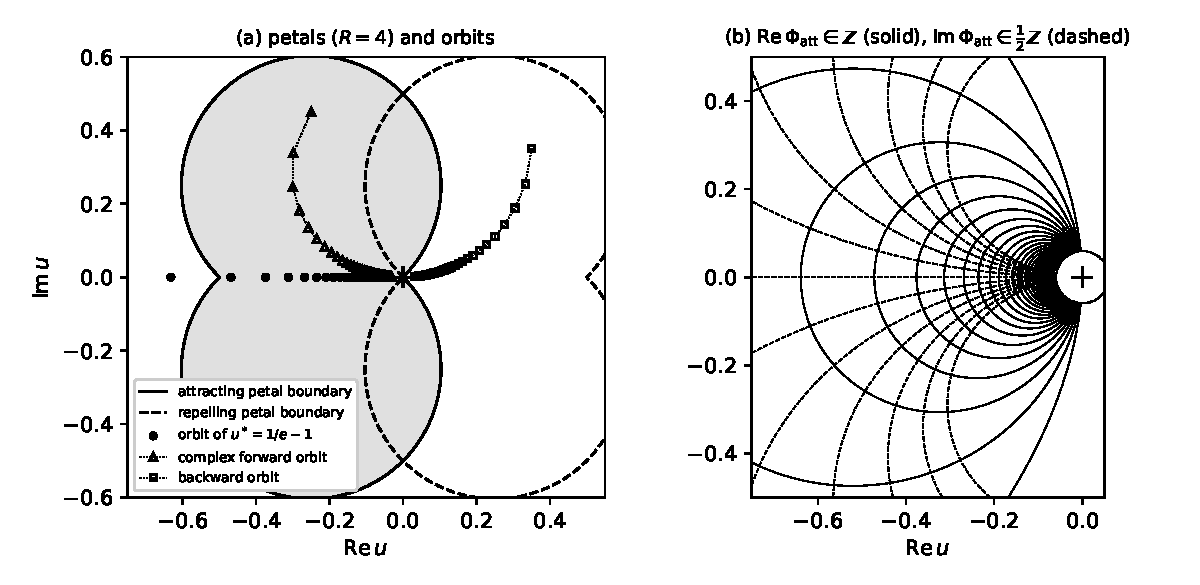
\includegraphics[width=\textwidth]{figures/fig3_petals.pdf}
\caption{$g(u)=\ee^u-1$。(a) 吸引花瓣（灰色，实线边界）与排斥花瓣（虚线边界），取示意值
$R=4$（$\zeta=-2/u$）；实心点是 $\ustar=1/\ee-1$ 的实轨道，三角是一条复轨道，二者沿负实轴切向趋于
$0$；方块是一条后向轨道，沿正实轴趋于 $0$。(b) $\Phiatt$ 的坐标网：实线 $\Rea\Phiatt\in\Z$，
虚线 $\Ima\Phiatt\in\frac12\Z$；相邻两条实线之间是 $g$ 的一个基本域。脚本
\texttt{figures/fig3\_petals.py}。}\label{ch3:fig:petals}
\end{figure}

%======================================================================
\notes

\paragraph{花瓣与 Fatou 坐标。} 花瓣定理属于 Leau（1897）与 Fatou \cite{Fatou1919}。
本章的证明在坐标 $\zeta=-1/(a_2u)$ 中把一切归结为「近似平移」$G(\zeta)=\zeta+1+O(1/\zeta)$，
这是 Milnor \cite[\S10]{Milnor2006} 与 Carleson--Gamelin \cite[第 II 章]{CarlesonGamelin1993}
的做法；我们只处理重数为 $2$ 的情形，此时只有一对花瓣，并且用 $s,t$ 两个线性函数给出了显式的
花瓣与增长率。Fatou 坐标用形式 Abel 函数归一化的写法见 Loray \cite{Loray2006} 与
Buff--Epstein \cite{BuffEpstein2002}；对 $\ee^u-1$ 的极限公式 $\Phiatt=\lim[\alpha(f^nu)-n]$
见 \cite[\S2.1]{KneserPaper}。迭代留数（résidu itératif）的名称来自 Écalle。

\paragraph{horn 映射与分类。} 解析分类定理属于 Écalle \cite{Ecalle1981} 与
Voronin \cite{Voronin1981}；「horn 映射」的名称来自复动力系统中的抛物内爆理论
（Douady、Lavaurs \cite{Lavaurs1989}、Shishikura \cite{Shishikura2000}）。
\Cref{ch3:thm:ecalle-voronin}(2) 的粘合证明是标准的；实现部分 (3) 我们只引用。不同文献对 horn
映射的方向（$\Phirep\circ\Phiatt^{-1}$ 还是其逆）、Fatou 坐标的加性常数、以及下 horn 映射常数项
的符号有不同的约定。本书的约定与论文一致：
$\horn^{-1}=\Phiatt\circ\Phirep^{-1}=z+\sum B_n\ee^{2\pi\ii nz}$，两侧都用 $\alpha$ 归一化。
论文把上 horn 映射的系数记为 $A_n$；本书改记为 $\tilde B_n$，以免与第 4 章的留数 $A_j$ 冲突。
论文 Remark~2.7 中柱面芽的系数与迭代留数也记作 $a_2,a_3,\rho$，本书记为 $\rho_H$。

\paragraph{$B_1\ne0$。} \Cref{prop:B1-nonzero} 的论证来自 \cite[Prop.~2.4、Remark~2.5]{KneserPaper}，
关键输入是 Chéritat 对单奇值类的抛物重整化 \cite{Cheritat2022}，背后的机制是 Epstein 的有限型
理论 \cite{Epstein1993}。近抛物重整化的另一套框架见 Inou--Shishikura \cite{InouShishikura}。

\paragraph{与论文的对应。} \cref{ch3:sec:fatou} 对应 \cite[\S2.1]{KneserPaper} 的前半与
\cite[\S4, Lemma~4.2、4.3]{KneserPaper} 在 $b=\eta$ 处的特例；\cref{ch3:prop:horn-expansion} 对应
\cite[\S4, (d)]{KneserPaper}；\cref{ch3:prop:normalisation}(3) 对应 \cite[Prop.~9.6]{KneserPaper}（基点无关性）在抛物侧的
部分；\cref{ch3:sec:examples} 的数值来自 \cite[\S2.1、Prop.~2.6、附录 A]{KneserPaper} 与
\texttt{docs/generality-check-zh.md} §2.1。论文的节号与定理号按投稿稿 \texttt{main.tex} 编译后的编号引用，对应源文件中的
标签 \texttt{sec:horn}、\texttt{eq:B12}、\texttt{prop:horn-nonzero}、\texttt{prop:horn-intervals}、
\texttt{rem:formal}、\texttt{sec:proofC}、注~9.5（\texttt{rem:gen-B1}） 为准。

%======================================================================
\exercises

\begin{exercise}\label{ch3:exe:mobius}
设 $g(u)=u/(1-u)$。验证 $\rho=0$，$\alpha(u)=-1/u$ 精确成立，$\Phiatt=\Phirep=-1/u$，
并且上、下 horn 映射都是恒等映射。
\end{exercise}

\begin{exercise}\label{ch3:exe:quadG}
对 $g(u)=u+u^2$ 验证 $G(\zeta)=\zeta+1+1/(\zeta-1)$，并据此对 $|\zeta|\ge4$ 给出\cref{ch3:lem:zeta}
中 $C_1$ 的一个显式值。
\end{exercise}

\begin{exercise}\label{ch3:exe:rho-iterate}
(1) 证明 $g^{\circ2}$ 的迭代留数是 $\rho/2$，更一般地 $g^{\circ m}$ 的是 $\rho/m$；并验证 $\alpha/m$
是 $g^{\circ m}$ 的形式 Abel 函数。(2) 证明 $\breve g(v):=-g^{-1}(-v)$ 是二重抛物芽，
$a_2(\breve g)=a_2$，$\rho(\breve g)=-\rho$。
\end{exercise}
\begin{hint}
(2) 用 \eqref{ch3:eq:ginv}。
\end{hint}

\begin{exercise}\label{ch3:exe:d1}
推导 \eqref{ch3:eq:d1}，并验证 $\ee^u-1$ 与 $u+u^2$ 的 $d_1$ 分别为 $-1/36$ 与 $-1/2$。
\end{exercise}

\begin{exercise}\label{ch3:exe:Btilde}
从 $\horn\circ\horn^{-1}=\id$ 推出 $\tilde B_3$ 用 $B_1,B_2,B_3$ 的表达式。
\end{exercise}

\begin{exercise}\label{ch3:exe:nonunique}
令 $\Phi=\Phiatt+\frac{1}{2\pi}\sin(2\pi\Phiatt)$。证明 $\Phi\circ g=\Phi+1$，但 $\Phi$ 不是 Fatou
坐标。\Cref{thm:fatou-coordinates}(4) 的哪个条件不成立？
\end{exercise}
\begin{hint}
由\cref{thm:fatou-coordinates}(3)，$\Ima\Phiatt$ 在 $\Patt(R)$ 上无界。
\end{hint}

\begin{exercise}\label{ch3:exe:real}
设 $g$ 是实芽。由\cref{thm:fatou-coordinates}(7)，$\Phiatt$ 在 $\Patt(R)\cap\R$ 上取实值。证明它在那里
严格递增；从而若 $\ustar<0$ 在直接吸引域的实区间中，则 $a=\Phiatt(\ustar)\in\R$。
\end{exercise}

\begin{exercise}\label{ch3:exe:orbit}
对 $\ee^u-1$ 与 $u_0=-1$，从\cref{ch3:cor:orbit} 推出\cref{ch3:ex:orbit} 中的极限
$2(a-1)-\tfrac23\log2$，并估计 $n=10^5$ 时的误差阶。
\end{exercise}

\begin{exercise}\label{ch3:exe:cylinder}
设 $B_1\ne0$，$H(q)=q\exp(2\pi\ii\sum_{n\ge1}B_nq^n)$。证明 $H$ 的迭代留数 $\rho_H$ 满足
$B_2/B_1^2=2\pi\ii(\tfrac12-\rho_H)$，并用\cref{ch3:tab:horn} 算出 $\ee^u-1$ 与 $u+u^2$ 的 $\rho_H$。
\end{exercise}

\begin{exercise}\label{ch3:exe:normal-form}
令 $X=\frac{a_2u^2}{1+\rho a_2u}\partial_u$，$\phi_X$ 为其时间一映射。
(1) 证明 $T(u)=-1/(a_2u)+\rho\log(-u)$ 满足 $T'=1/X$，从而 $T\circ\phi_X=T+1$，$\phi_X$ 的
迭代留数为 $\rho$。(2) 证明存在形式变换 $h(u)=u+O(u^2)$ 使 $T\circ h=\alpha+\mathrm{const}$，并由此
推出 $h\circ g=\phi_X\circ h$（形式上）。(3) 证明 $\phi_X$ 的上、下逆 horn 映射分别为 $z$ 与
$z+2\pi\ii\rho$。
\end{exercise}
\begin{hint}
(2) 比较 $T(u(1+h_1u+h_2u^2+\cdots))$ 与 $\alpha(u)$ 的 $u^{k-1}$ 项：$h_k$ 以系数 $1/a_2$ 出现，其余
只含 $h_1,\dots,h_{k-1}$。(3) $T$ 在两片花瓣上就是 Fatou 坐标。
\end{hint}

\begin{exercise}\label{ch3:exe:embed}
（较难）证明：若 $B_n=0$ 且 $B_{-n}=0$ 对所有 $n\ge1$ 成立，则 $g$ 解析共轭于习题~\ref{ch3:exe:normal-form}
中的 $\phi_X$，从而 $g$ 可以嵌入一个全纯向量场的流。
\end{exercise}
\begin{hint}
用\cref{ch3:thm:ecalle-voronin}(2)，取 $g_1=\phi_X$，$\kappa=0$。
\end{hint}

\begin{exercise}\label{ch3:exe:residue-analytic}
（较难）不经过形式计算，直接证明 $\rho$ 是解析共轭不变量：对任意使 $\Phirep$ 在 $\Prep(R)$ 上单值的
归一化，上、下逆 horn 映射的常数项之差都等于 $2\pi\ii\rho$。
\end{exercise}
\begin{hint}
常数项之差在 $\Phiatt\mapsto\Phiatt+c_{\mathrm a}$、$\Phirep\mapsto\Phirep+c_{\mathrm r}$ 下不变（\cref{ch3:prop:normalisation}(1)）。
对 $\alpha_0$ 归一化的坐标，用 \eqref{ch3:eq:same-alpha}。
\end{hint}
